\documentclass[11pt,a4paper]{article}
% Built by scripts/paper/build_manuscript_tex.py from the manuscript .txt source. Do not edit by hand:
% edit the .txt and rebuild, so that the .docx and the .tex stay identical in content.
\usepackage{iftex}
\ifPDFTeX
  \usepackage[utf8]{inputenc}
  \usepackage[T1]{fontenc}
  \usepackage{lmodern}
\else
  \usepackage{fontspec}
\fi
\usepackage[margin=1in]{geometry}
\usepackage{amsmath,amssymb}
\usepackage{graphicx}
\usepackage{booktabs,tabularx,rotating}
\usepackage{xcolor}
\usepackage[numbers,sort&compress]{natbib}
\usepackage[hidelinks]{hyperref}
\usepackage{microtype}
\graphicspath{{figures/}}
\newcommand{\pending}[1]{\textcolor{red}{\textbf{#1}}}
\setlength{\emergencystretch}{3em}

\title{The Inertia Problem in a Fine-Tuned Vision-Language-Action Driving Policy: A Closed-Loop Comparison of Checkpoints Trained on Different Data Mixes}
\author{\pending{[[PENDING: authors and affiliations]]}}
\date{}

\begin{document}
\maketitle

\begin{abstract}
Imitation-learned driving policies can learn that a vehicle at rest stays at rest, the inertia problem. We ask whether checkpoints of a vision-language-action policy fine-tuned on different data mixes differ in this behaviour. In a single-seed study we fine-tuned the flow-matching action expert of Alpamayo 1.5 on a balanced mix and on an obstacle-heavy mix with more stationary samples, drawn from one pool of CARLA expert data on the same schedule, and evaluated the checkpoints in closed loop on 44 Bench2Drive routes. At 6,400 samples the obstacle-heavy checkpoint returned a near-stationary plan (a planned path shorter than 1.5 m, the threshold of the controller's standstill gate) in 26.80 \% of steps, the balanced checkpoint in 1.31 \% (pre-specified test: \ensuremath{-}25.49 percentage points, 95 \% CI [\ensuremath{-}31.69, \ensuremath{-}19.63]) and the unadapted policy in 13.24 \%. The difference recurred in a second pass and, in the same direction, on identical replayed inputs. The balanced checkpoint stood still about half as long and completed more of each route. It also spent more time commanded to accelerate without moving. Its Driving Score was not detectably higher (+3.96 points, CI [\ensuremath{-}3.06, 11.67]), and its collision events per route did not differ detectably (+0.24, CI [0.00, 0.43]; 28 against 28 events in the first pass and 36 against 15 in the second). Post hoc, its Bench2Drive Driving Efficiency was higher (+22.89 points, CI [6.14, 34.89]); the test of this measure at 1,600 samples, fixed before its values were computed, was not met. In an exploratory run without the standstill gate the difference in full stops shrank to \ensuremath{-}4.65 percentage points (CI [\ensuremath{-}11.44, 3.20]), while the difference in plans remained. A third checkpoint, which separates the scenario-group shares from the manoeuvre mix and the stationary share, returned near-stationary plans about as rarely as the balanced one (1.58 \% of steps). At 1,600 samples the differences were small and at the border of detection. In an exploratory test, replacing the ego-motion history of the obstacle-heavy checkpoint changed its planned accelerations; the test does not identify a mechanism. One pass of the 44 routes was not enough to compare checkpoints on Driving Score. Variation between training runs is untested, no stop is shown to be unwarranted, and we make no safety claim.
\end{abstract}

\textbf{Keywords:} vision-language-action models; flow matching; imitation learning; fine-tuning data composition; low-speed planning; closed-loop evaluation; autonomous driving

\section{Introduction}

Vision-Language-Action (VLA) models for driving combine a pretrained vision-language model (VLM), which encodes camera images, ego-motion history and a navigation instruction, with an action head that outputs a future trajectory. In designs that pair a VLM with a separate action expert, such as $\pi_0$ \cite{ref26}, $\pi_{0.5}$ \cite{ref1} and NVIDIA's Alpamayo family \cite{ref2,ref19}, the action head is a continuous flow-matching \cite{ref8} expert that turns a noise sample into a trajectory in a few solver steps. Unlike a regression head, it can represent several distinct futures for one scene and returns one of them at each call.

Such a policy is commonly adapted to a new simulator or vehicle by supervised fine-tuning of the action expert with the VLM frozen. The practitioner then decides what the fine-tuning set contains. A natural instinct is to add more of what is hard: obstacles, hazards, emergency stops. In the obstacle-heavy mix we study, the share of stationary samples was also set higher, and among its low-speed samples the expert stays put in 31 \%, against 11 \% in the balanced mix. Whether this share changes what the fine-tuned policy plans is the question of this study. Standing still when the road is clear and making contact with an obstacle are two different failures. We measure both, assume no relation between them, and cannot place either checkpoint relative to safety.

Imitation-learned driving policies that observe their own motion can learn that a vehicle at rest tends to stay at rest. Codevilla et al. \cite{ref12} named this the inertia problem; it is a form of causal confusion \cite{ref13} and of the copycat behaviour described for policies trained on observation histories \cite{ref25,ref28}. The remedies proposed so far act on the model input, the loss or the weighting of training frames \cite{ref12,ref27,ref28}. Outside driving, robot policies have been reported to freeze or idle because of what their training data contain \cite{ref44,ref45}. In driving, training on generated safety-critical scenarios has been reported to improve collision avoidance \cite{ref38}, and re-weighting or rebalancing of training samples to raise benchmark scores \cite{ref33,ref39}; Alpamayo 1.5 has been reported to get stuck in CARLA \cite{ref34}.

We have not found a study that changes only the composition of the fine-tuning set of such a policy, holds the model, the loss, the training schedule and the controller fixed, and measures the result in closed loop at the level of the plans the model produces. Without the last step the question cannot be answered, because standstill in closed loop is a joint product of the model and of the controller that executes its plans.

We fine-tuned the 2.28B-parameter action expert of Alpamayo 1.5 on two mixes drawn from one verified pool of CARLA expert samples. The balanced mix (\texttt{Golden}) targets 50 \% straight driving, symmetric lateral manoeuvres and 2 \% stationary samples; the obstacle-heavy mix (\texttt{Flooded}) targets a larger share of obstacle and hazard scenario groups, a left-skewed lateral distribution and 10 \% stationary samples. Each is built at 1,600 and 6,400 samples, with identical training schedules at each size, and the models are evaluated in closed loop on 44 Bench2Drive routes \cite{ref3}. We then repeated the evaluation of both 6,400-sample models, ran both with the controller's standstill gate removed, analysed the logged plan of every step, trained a third checkpoint that separates one of the three factors in which the mixes differ, and tested whether the plans depend on the ego-motion history.

The study has four tests; Section 4.1 states when each was fixed.

\begin{itemize}
\item \textbf{Plans (primary):} at 6,400 samples and a matched training schedule, the balanced-mix checkpoint (\texttt{Golden\mbox{-}6400}) returns a near-stationary plan, with a predicted path shorter than 1.5 m, in a smaller share of steps than the obstacle-heavy-mix checkpoint (\texttt{Flooded\mbox{-}6400}).
\item \textbf{Standstill time:} \texttt{Golden\mbox{-}6400} spends less route time below 0.1 m/s than \texttt{Flooded\mbox{-}6400}.
\item \textbf{Repeat test:} in a second pass of the same two checkpoints the difference in near-stationary plans recurs, as do the differences in blocked time (time at rest while the controller commands acceleration) and in the standstill outside it.
\item \textbf{Dataset size:} the difference in near-stationary plans is also present at 1,600 samples.
\end{itemize}

The first three were fixed before any of their runs. The fourth was fixed while its second run was in progress, before any value of either run was computed. The readings of four further analyses were also fixed before their data: the same-input replay, the decoupling checkpoint, the run without the gate and the history-swap test. Each of the four had been run once in the preliminary evaluations, with its outcome known, and its rule was not changed. All other analyses are labelled post hoc or exploratory.

We found four things.

\begin{itemize}
\item \textbf{The two checkpoints differed strongly in how often they returned a near-stationary plan.} \texttt{Flooded\mbox{-}6400} returned a near-stationary plan in 26.80 \% of steps and \texttt{Golden\mbox{-}6400} in 1.31 \% (pre-specified test: \ensuremath{-}25.49 percentage points, 95 \% CI [\ensuremath{-}31.69, \ensuremath{-}19.63]), and the difference recurred in a second pass (\ensuremath{-}28.16 pp, CI [\ensuremath{-}34.81, \ensuremath{-}21.75]). On identical replayed inputs the stay-put share was 17.61 \% against 0.35 \%, with the unadapted policy between the two at 3.28 \% (Section 4.2), so the difference belongs to the experts and not only to the states each of them reached. In closed loop the unadapted policy returned a near-stationary plan in 13.24 \% of steps (Section 4.7). The 1.5 m threshold is that of the controller's standstill gate, so the closed-loop rate is taken with the gate active; without the gate the same two checkpoints returned such a plan in 14.58 \% and 0.60 \% of steps (Section 4.4). A third checkpoint, trained on the scenario-group shares of the obstacle-heavy set with the manoeuvre mix and stationary share of the balanced set, returned near-stationary plans about as rarely as the balanced one (1.58 \% of steps against 1.22 \%; Section 4.5). At 1,600 samples the difference was far smaller and at the border of detection (8.34 \% against 4.92 \%; \ensuremath{-}3.42 pp, CI [\ensuremath{-}7.74, \ensuremath{-}0.11], p = 0.047; Section 4.6).
\item \textbf{The behaviour matches the description of the inertia problem \cite{ref12}; we do not show that the stops were unwarranted.} The checkpoint trained on more stationary samples stayed put more often once slow, which is the behaviour that Codevilla et al. describe. Our logs do not show whether a given stop was required, and on the replayed states the balanced checkpoint stayed put less often than the expert demonstrations did (0.63 \% of plans against 3.91 \% of demonstrated futures, both pooled over the 384 states; Section 4.2), so staying put less is not shown to be better.
\item \textbf{In an exploratory test, the planned accelerations of the obstacle-heavy checkpoint depended on its ego-motion history.} The test, on six routes, replaced the ego history of \texttt{Flooded\mbox{-}6400} at low speed by one that reports motion; the share of plans that hold their speed rose by 32.00 pp (CI [22.63, 36.04]; Section 4.8). By the rule fixed in advance, the learned controls of this checkpoint depend on its ego history. The test does not identify the mechanism: the rule's condition for tying the stay-put plans to a history that reports rest was not met, a policy that uses its speed correctly could give the same outcome, and the camera input was not varied.
\item \textbf{Less standstill came with more progress and more blocked time, not with a higher Driving Score; collision events did not differ detectably.} Over both passes \texttt{Golden\mbox{-}6400} stood still about half as long (\ensuremath{-}23.54 pp, CI [\ensuremath{-}32.98, \ensuremath{-}14.89]) and completed more of each route (+6.84 pp, CI [0.80, 13.29]). It also spent more time commanded to accelerate without moving (+14.29 pp, CI [7.57, 24.21]), and its Driving Score was not detectably higher (+3.96 points, CI [\ensuremath{-}3.06, 11.67]). Its collision events per route did not differ detectably (0.73 against 0.49; +0.24, CI [0.00, 0.43]; 28 against 28 events in the first pass and 36 against 15 in the second), nor did its collision events per distance driven (ratio 1.29, CI [0.90, 1.92]). Without the controller's standstill gate the difference in full stops shrank to \ensuremath{-}4.65 pp (CI [\ensuremath{-}11.44, 3.20]), while the difference in near-stationary plans (\ensuremath{-}13.99 pp, CI [\ensuremath{-}20.27, \ensuremath{-}9.52]) and in slow driving remained (Section 4.4), which supports an origin of the difference in the plans, with the gate turning short plans into held stops (exploratory, one pass). We make no safety claim in either direction.
\end{itemize}

The paper contributes (i) a controlled comparison of the low-speed behaviour of checkpoints of one flow-matching VLA driving policy that were fine-tuned once each on different data compositions, with the model, loss, schedule and controller held fixed; (ii) measures at the level of the plan, the motion and the command (stay-put plans by speed, crawling, blocked time) that separate what the model plans from what the controller makes of it, with a same-input replay and a closed-loop run without the gate to check them; (iii) the observation that, in this pair, the checkpoint that stood still less made more progress, spent more time blocked and did not obtain a detectably higher Driving Score; (iv) a loading check for serving fine-tuned action experts with the FlashDrive inference engine \cite{ref15}, which otherwise leaves part of the fine-tuned weights unloaded without an error (Section 3.4). The five datasets are released (Section 6).

The limits are those of the design: one training seed per condition, two mixes that differ in three factors at once (the third checkpoint separates one of them), one policy, one simulator, 44 routes and a controller tuned on 20 of them. With one training run per mix, the dependence on composition across training runs is untested, and a second evaluation pass addresses evaluation noise, not variation between training runs. At 1,600 samples the difference in plans was small and did not detectably reach standstill time (Section 4.6).

\section{Related Work}

End-to-end driving and language. Camera--LiDAR fusion by transformer attention \cite{ref21}, reinforcement-learning coaches for imitation agents \cite{ref22}, planning-oriented multi-task networks \cite{ref4}, vectorized scene representations \cite{ref5} and multi-teacher trajectory scoring \cite{ref23} have each raised driving benchmarks; these planners output a trajectory by regression or by scoring candidates. DriveLM \cite{ref6} casts driving as graph-structured question answering, LMDrive \cite{ref7} conditions closed-loop control on language instructions, and SimLingo \cite{ref24} aligns language and actions in a vision-only model evaluated on Bench2Drive. Alpamayo-R1 \cite{ref2} and Alpamayo 1.5 \cite{ref19} combine chain-of-causation reasoning with a flow-matching action expert; we use the latter.

Generative action heads. Diffusion Policy \cite{ref29} models robot action sequences with conditional denoising diffusion, and DiffusionDrive \cite{ref30} adapts truncated diffusion with anchor trajectories to end-to-end driving. $\pi_0$ \cite{ref26} attaches a flow-matching action expert to a pretrained VLM. Flow matching \cite{ref8} regresses a velocity field along a probability path; with a linear path and independent noise--data coupling the learned paths are not straight in general, and straighter paths need additional procedures \cite{ref31,ref32}. These heads can represent several modes; the question we ask is which mode they sample at low speed.

Inertia, copycat behaviour and their mitigations. Codevilla et al. \cite{ref12} documented the inertia problem in behaviour cloning for driving and proposed an auxiliary speed-prediction branch. de Haan et al. \cite{ref13} framed the broader failure as causal confusion. Wen et al. \cite{ref25} analysed copycat agents that exploit observation histories; their keyframe method \cite{ref28} upweights demonstration frames at expert action changes. ChauffeurNet \cite{ref27} applied dropout to the past-motion input during training. Open-loop planning metrics on nuScenes \cite{ref11} can be matched by models that use only ego status \cite{ref17,ref18}, which is the same shortcut seen from the evaluation side. Closed-loop agents can also include controller-side rules for leaving rest; Jaeger et al. \cite{ref40} note that waypoint-predicting models need controller heuristics when stopped. All of these remedies act on the model input, the loss, the weighting of training frames or the controller. Our intervention acts only on the composition of the fine-tuning set. We did not run a history-dropout baseline or a creep-rule controller, so we cannot say how a data-side change compares with them (Section 5).

Idling, freezing and over-caution. Kim et al. \cite{ref44} report that all-zero actions in a robot dataset led a vision-language-action policy to freeze during evaluation, and they removed those actions from the training data. Chen et al. \cite{ref45} describe policy idling in dexterous manipulation as often a reflection of the training data. In motion planning, the freezing robot problem \cite{ref49,ref42} denotes a planner that judges every forward path through a dense crowd unsafe and stops, and Sadigh et al. \cite{ref43} observe that planners which only stay out of the way of predicted human trajectories tend toward defensive behaviour. For end-to-end driving in CARLA, Jaeger et al. \cite{ref40} identify a bias in which multimodal waypoint predictions are averaged longitudinally and the vehicle slows down, and Chuang et al. \cite{ref41} address the copycat problem with a residual action target. These works locate the tendency to stop in the data, in the output representation or in the planner.

Composition of imitation data. Belkhale et al. \cite{ref36} characterise the quality of an imitation dataset by action divergence and transition diversity. Hejna et al. \cite{ref35} learn the weights of a mixture of robot datasets and report that the learned weights outperform uniform and hand-chosen ones. Xing et al. \cite{ref46} trace shortcut learning in generalist robot policies to limited diversity within sub-datasets and to distribution gaps between them. In driving, Hanselmann et al. \cite{ref38} show that training on generated safety-critical scenarios improves collision avoidance, Mirkhani et al. \cite{ref39} reweight training samples by learned clusters and report closed-loop gains on Bench2Drive, and Zimmerlin et al. \cite{ref37} find that the style of the expert significantly affects the trained policy. Wang et al. \cite{ref33} find that reweighting the training data by trajectory pattern is effective for a flow-matching planner on nuPlan and interPlan; their planner has no vision-language model, and they report benchmark scores, not standstill. Nguyen et al. \cite{ref34} evaluate off-the-shelf vision-language-action driving models in CARLA 0.9.15 and report that Alpamayo 1.5 tends to get stuck on one of their routes. These studies ask whether a change of data improves a benchmark score. We have not found a controlled change of the fine-tuning mix for such a model with low-speed behaviour in closed loop as the endpoint and the controller's part separated. Que et al. \cite{ref48} report, for a camera-only planner on Bench2Drive with one seed, that 26 of 42 blocked routes ended with a learned brake output holding the vehicle while the planned trajectory asked for motion; a rule that released this hold reduced the blocked routes from 41 to 24 on the routes common to both runs and raised vehicle collisions from 0.44 to 0.62 per route, without a clear change in Driving Score. That study varies the controller-side rule on one model; ours holds the controller fixed and varies the fine-tuning data, and removes the hold as an ablation.

Closed-loop evaluation. Errors of an imitation policy compound in closed loop \cite{ref16}, and open-loop planning metrics do not show this \cite{ref17,ref18}. CARLA \cite{ref9} executes the policy's commands at every tick; repeated executions of the same scenario in it are not identical, and Chance et al. \cite{ref47} study this variance and the conditions under which it becomes negligible. Bench2Drive \cite{ref3} splits closed-loop evaluation into 220 short routes covering 44 scenario types and five abilities (Merging, Overtaking, Emergency Braking, Give Way, Traffic Signs). LEAD \cite{ref10} reduces learner--expert asymmetries in CARLA expert data; our demonstrations come from the LEAD expert.

\section{Methodology}

\subsection{Problem Formulation and Dual-System Architecture}

At control step $t$ the policy receives $\mathbf{x}_t = (\mathcal{I}_t, \mathcal{H}_t, c_t)$:

\begin{enumerate}
\item[1.] \textbf{Cameras:} $\mathcal{I}_t$ from four cameras (cross-left, front-wide and cross-right at $120^\circ$ field of view; front-telephoto at $30^\circ$) over a 4-frame window \cite{ref19}.
\item[2.] \textbf{Ego-motion history:} $\mathcal{H}_t = \{(\mathbf{p}_i, \mathbf{R}_i)\}_{i=0}^{15}$, 16 poses at $\Delta t = 0.1\text{ s}$ spacing over the last $1.5\text{ s}$ (the last pose is the current one), in the current ego frame ($x$ forward, $y$ left), tokenized into 48 history tokens (three per pose) that form part of the VLM input \cite{ref2,ref19}.
\item[3.] \textbf{Navigation instruction:} $c_t$, a short text such as \texttt{Continue straight} or \texttt{Turn left in 11m} \cite{ref19}.
\end{enumerate}

The policy outputs $K = 64$ future waypoints at the same $\Delta t = 0.1\text{ s}$ spacing ($6.4\text{ s}$ horizon; the first waypoint is $0.1\text{ s}$ ahead of the current pose), $\mathbf{W} = [\mathbf{w}_1, \dots, \mathbf{w}_K]^\top$, $\mathbf{w}_k = (x_k, y_k, z_k)$, in the ego frame at time $t$ \cite{ref2,ref19}. The vertical coordinate is not modelled; it is set to the current ego height.

Alpamayo 1.5 (about 10B parameters) consists of an 8B-parameter VLM backbone $\Phi_{\text{VLM}}$ (\nolinkurl{nvidia/Cosmos-Reason2-8B}, Qwen3-VL architecture), which encodes $\mathbf{x}_t$ (the ego history included, as tokens) into a cached key-value state $\mathbf{e}_t$, and a 2.28B-parameter action expert $v_\theta$ that works in a unicycle acceleration--curvature action space \cite{ref2,ref19}. A trajectory is represented by normalized controls $\mathbf{A}_1 = [\mathbf{u}_1, \dots, \mathbf{u}_K]^\top \in \mathbb{R}^{K \times 2}$, $\mathbf{u}_k = \big((a_k - \mu_a)/\sigma_a,\, (\kappa_k - \mu_\kappa)/\sigma_\kappa\big)$ for acceleration $a_k$ and curvature $\kappa_k$, with $(\mu_a, \sigma_a) = (0.0290, 0.6810)\text{ m/s}^2$ and $(\mu_\kappa, \sigma_\kappa) = (0.000269, 0.0261)\text{ m}^{-1}$. Controls are mapped to waypoints by unicycle integration with trapezoidal quadrature \cite{ref2,ref19}, starting at the ego origin with zero heading and at an initial speed $v_0$ that the model estimates from $\mathcal{H}_t$ (it is not a learned output):

\[
v_k = v_0 + \sum_{j=1}^{k} a_j \Delta t, \quad \psi_k = \sum_{j=1}^{k} \kappa_j \left(v_{j-1}\Delta t + \tfrac{1}{2}a_j \Delta t^2\right)
\]

\[
x_k = \sum_{j=1}^{k} \tfrac{\Delta t}{2}\big(v_{j-1}\cos\psi_{j-1} + v_j\cos\psi_j\big), \quad y_k = \sum_{j=1}^{k} \tfrac{\Delta t}{2}\big(v_{j-1}\sin\psi_{j-1} + v_j\sin\psi_j\big)
\]

We call $L = \sum_{k=2}^{K} \lVert (x_k, y_k) - (x_{k-1}, y_{k-1}) \rVert_2$ the predicted trajectory extent: the planar path length from the first to the last waypoint (63 segments; the first segment, from the ego position to the first waypoint and about $v_0 \Delta t$ long, is not included, in the controller and in every analysis below). Because the integration starts at $v_0$, $L$ depends on the current speed as well as on the learned controls: with every control at its training mean, a plan from rest has $L = 0.59\text{ m}$, and a plan from $v_0 = 0.4\text{ m/s}$ has $L = 3.1\text{ m}$. Statements about $L$ at low speed therefore condition on speed (Section 4.3). Supplementary Section S3.1 gives a numerical check of these equations.

The action expert is trained by conditional flow matching with a linear interpolation path and independent coupling \cite{ref8}: $\mathbf{A}_0 \sim \mathcal{N}(\mathbf{0}, \mathbf{I})$ is drawn independently of the demonstration $\mathbf{A}_1$, $\mathbf{A}_s = (1-s)\mathbf{A}_0 + s\mathbf{A}_1$ for $s \in [0,1]$, and the network regresses the conditional velocity $\mathbf{A}_1 - \mathbf{A}_0$:

\[
\mathcal{L}_{\text{CFM}}(\theta) = \mathbb{E}_{s \sim p(s),\, \mathbf{A}_0,\, (\mathbf{x}_t, \mathbf{A}_1) \sim \mathcal{D}} \left[ \lVert v_\theta(\mathbf{A}_s, s \mid \mathbf{e}_t) - (\mathbf{A}_1 - \mathbf{A}_0) \rVert_2^2 \right]
\]

Here $p(s)$ is the flow-time distribution of the training recipe \cite{ref20}, which we did not change (\cite{ref2} describes a shifted beta distribution; we did not verify the distribution in the recipe version we ran). At inference the expert integrates $d\mathbf{A}_s/ds = v_\theta(\mathbf{A}_s, s \mid \mathbf{e}_t)$ from a noise sample at $s = 0$ to $s = 1$. The expert sees the ego history only through $\mathbf{e}_t$; the history acts a second time through $v_0$ in the integration above.

\subsection{Why Data Composition Could Change Low-Speed Plans: A Sampling Conjecture}

The minimiser of $\mathcal{L}_{\text{CFM}}$ is the marginal velocity field, and integrating it from Gaussian noise transports the noise distribution to the training conditional $p_{\text{train}}(\mathbf{A}_1 \mid \mathbf{e}_t)$ in the limit of exact fit and exact integration \cite{ref8}. In that limit each inference call returns a sample from the conditional distribution, not its mean. If the training data contain a mixture of futures in a given context, a well-fitted expert returns each kind about as often as the data do, so changing the composition changes how often each is sampled. The deployed sampler is far from the limit: it evaluates the expert four times per call (Section 3.4), and a coarse integration can pull samples toward the conditional mean. That is a rival mechanism for short plans, and we did not test it.

The relevant contexts are low-speed ones, where the camera image and the ego history are often compatible both with staying put and with starting to move. For samples with ego speed $\le 0.5\text{ m/s}$ we define three classes of future by the path length $L$ of the $6.4\text{ s}$ trajectory: stays put ($L < 0.64\text{ m}$, a planned mean speed below $0.1\text{ m/s}$), starts moving ($L \ge 2\text{ m}$), and in between.

\textbf{Conjecture (stay-put sampling).} A flow-matching expert trained on data in which a larger share of low-speed samples stay put will, in low-speed closed-loop contexts, sample stay-put trajectories more often. Because the vehicle then remains at low speed, the next query again sees a low-speed context, so repeated stay-put samples extend the time at rest after the reason for stopping has gone.

The conjecture is not one of the tests of this study. It was formulated after first closed-loop results of these checkpoints were known, so their agreement with it is not a test of it. The relevant share is the conditional one among low-speed samples, not the global stationary share (Table 1): 30.9 \% of low-speed samples stay put in the obstacle-heavy 6,400-sample set and 10.9 \% in the balanced one; at 1,600 samples the shares are 30.6 \% and 11.4 \%. The conjecture does not predict the 1,600-sample result, where the shares differ almost as much and the checkpoints differ far less (Section 4.6), so it is at most part of the explanation. The shares are marginal shares over all low-speed samples; the conjecture needs in addition that the frozen backbone often cannot tell the contexts in which the expert stays from those in which it starts, and we did not measure this. A second reading of the 1,600-sample result is that fine-tuning moves the expert away from its pretrained behaviour gradually, so that 2,000 optimizer steps change the plans less than 8,000; the design cannot separate the number of steps from the number of samples. The lateral asymmetry of the obstacle-heavy mix is a rival explanation for stay-put plans on obstacle-bypass routes, and the design cannot separate the two. Supplementary Section S3.2 gives the argument in full.

\subsection{Fine-Tuning Datasets}

Demonstrations come from the LEAD \cite{ref10} privileged expert, recorded in CARLA 0.9.16 at rendering quality Epic and converted to the PhysicalAI-AV layout. A route enters the verified pool only if the expert completed it fully and without a disqualifying infraction. The four datasets of the main design, two mixes at two sizes, are drawn from one verified training pool; we call them the Matrix datasets (\texttt{lead\_multirig\_pai\_v4}, 34,132 samples at a 0.4 s stride; 1,840 clips over 646 routes). Each sample is labelled with a scenario group (A--F; obstacle avoidance and construction, junctions, hazards and emergencies, highway and merging, vulnerable road users and dynamic conflicts, baseline and signal compliance) and a navigation manoeuvre (straight, swerve left, swerve right, turn left, turn right). A sample is stationary if the ego vehicle moves less than 0.5 m over its 6.4 s future.

Each mix, or regime, is specified by target marginals: the group shares, the manoeuvre shares and the stationary share (Table 1). The group \ensuremath{\times} manoeuvre allocation is an iterative proportional fit of the pool's own counts onto the target marginals, and samples are then selected deterministically. Each 1,600-sample set is the exact per-bucket first quarter of the 6,400-sample set of the same regime. The balanced and obstacle-heavy 6,400-sample sets share 4,284 samples (66.9 \% of each). All datasets share one validation split of 1,567 samples.

The two regimes differ in three factors at once (group mix, lateral balance and stationary share), and in this pool the factors are coupled: groups A and C hold 88 \% of all left swerves but 58 \% of right swerves, so raising the hazard share pushes the lateral balance left. Comparisons between regimes therefore estimate the effect of the bundle. A fifth dataset, \texttt{floodedgroups\_balanced\_6400} (the scenario-group shares of the obstacle-heavy mix with the manoeuvre shares and the 2 \% stationary share of the balanced mix; we call it the decoupling mix), separates the group mix from the lateral-plus-stationary bundle. One model, \texttt{Decoupling\mbox{-}6400}, was trained on it with the recipe and schedule of the other 6,400-sample models; its evaluation is reported in Section 4.5. The decoupling set shares 5,523 of its 6,400 samples (86.3 \%) with the balanced 6,400-sample set and 4,112 (64.3 \%) with the obstacle-heavy one.

Training and evaluation routes overlap. Mapped exactly to the 44 evaluation routes we use, training samples in the Matrix sets touch seven routes; the number of touching samples is 20 (golden\_1600), 19 (flooded\_1600), 78 (golden\_6400) and 87 (flooded\_6400). Because the overlap is of similar size in both regimes, it bears mainly on comparisons against the unadapted Alpamayo 1.5, which we call \texttt{Base}. Section 4.3 gives the two main contrasts on the 37 routes not touched by training samples. Supplementary Section S3.3 gives the construction and the overlap in full.

\begin{table}[htbp]
\small
\caption{Composition of the fine-tuning datasets (targets equal realised values for all five sets; for the decoupling set the realised group and manoeuvre shares are those of its dataset card and annotations). The low-speed counts of the 6,400-sample sets are taken from the published annotations; those of the 1,600-sample sets come from the training provenance record, whose counts for the 6,400-sample sets differ from the published annotations by at most five samples. Pool v4 is \texttt{lead\_multirig\_pai\_v4}; dataset names are the last part of the Hugging Face names in Section 6.}
\begin{tabularx}{\linewidth}{>{\raggedright\arraybackslash}X>{\raggedright\arraybackslash}X>{\raggedright\arraybackslash}X>{\raggedright\arraybackslash}X}
\toprule
\textbf{Property} & \textbf{\texttt{Flooded} (1,600 / 6,400)} & \textbf{\texttt{Golden} (1,600 / 6,400)} & \textbf{\texttt{Decoupling} (6,400)} \\
\midrule
Source pool & pool v4, 34,132 samples & pool v4, 34,132 samples & pool v4 \\
Groups A / B / C / D / E / F (\%) & 35 / 14 / 22 / 10 / 9 / 10 & 27 / 18 / 17 / 14 / 14 / 10 & 35 / 14 / 22 / 10 / 9 / 10 (realised; the target of \texttt{Flooded}) \\
Straight / swerve L / swerve R / turn L / turn R (\%) & 22 / 37 / 12 / 14.5 / 14.5 & 50 / 13 / 13 / 12 / 12 & 50 / 13 / 13 / 12 / 12 \\
Stationary samples (\%) & 10 (160 / 640) & 2 (32 / 128) & 2 (128) \\
Brake / hazard share at 6,400 (\%, observed) & 41.3 / 30.8 & 35.4 / 23.8 & 35.1 / 24.2 \\
Samples at \ensuremath{\leq} 0.5 m/s, 1,600 set: stay put / start / between & 168 / 346 / 35 of 549 (30.6 \% stay put) & 44 / 302 / 41 of 387 (11.4 \% stay put) & no 1,600 set \\
Samples at \ensuremath{\leq} 0.5 m/s, 6,400 set: stay put / start / between & 663 / 1,343 / 137 of 2,143 (30.9 \% stay put) & 171 / 1,251 / 148 of 1,570 (10.9 \% stay put) & 167 / 1,210 / 130 of 1,507 (11.1 \% stay put) \\
Training samples touching the 44 evaluation routes & 19 / 87 & 20 / 78 & not computed \\
Hugging Face dataset & \texttt{flooded\_1600}, \texttt{flooded\_6400} & \texttt{golden\_1600}, \texttt{golden\_6400} & \texttt{floodedgroups\_} \texttt{balanced\_6400} \\
\bottomrule
\end{tabularx}
\end{table}

\subsection{Fine-Tuning, Inference and Controller}

Parameter isolation. The VLM backbone is frozen during fine-tuning \cite{ref2,ref20}; only the action expert is trained (2,280,592,386 parameters according to the trainer artifacts). Training follows the Alpamayo Stage-2 recipe \cite{ref20} (AdamW, gradient-norm clipping at 1.0, \texttt{bfloat16}, cosine schedule from $10^{-4}$ to $10^{-6}$) and ran on an NVIDIA A100 machine. For deployment on one 24 GB GPU the frozen VLM language layers are quantized to 4-bit weights with pairwise rotation quantization (ParoQuant) \cite{ref14} and run with 8-bit activations in the FlashDrive streaming server \cite{ref15}; the action expert runs in \texttt{bfloat16}.

Schedules. All four Matrix models and the decoupling model used per-device batch 1 with gradient accumulation 8 (effective batch 8), 10 epochs and seed 42. This gives 2,000 optimizer steps at 1,600 samples and 8,000 at 6,400 samples. The configurations of the two 6,400-sample Matrix models are identical except for the dataset name, and both trained without interruption. The two 1,600-sample models share a schedule but were each interrupted and resumed from a saved checkpoint. Table S1 gives the training and evaluation provenance of every checkpoint.

Inference. The FlashDrive server \cite{ref15} keeps a sliding-window key-value cache and integrates the learned field in eight uniform forward-Euler steps. In the server code we ran, the velocity is reused, not recomputed, on four of the eight steps, so the expert is evaluated four times per call. We did not measure the discretisation error. The model server does not seed its noise draws, so each inference call uses fresh noise and closed-loop runs are not reproducible step for step (Section 4.1). CARLA runs synchronously at 20 Hz. The agent queries the server at every 20 Hz simulator step and acts on the plan it returns; no plan is held over several steps.

Loading of the fine-tuned expert. The stock server first loads the base model and then copies the tensors of a fine-tuned action expert into it by name; names that find no match are skipped. When the base model is loaded, the inference engine merges the query, key and value projections of each of the 36 expert layers into one tensor, and the gate and up projections of each feed-forward block into another. A checkpoint stores these five projections separately, so their names match nothing and they are skipped without a message: 180 of the 396 expert-layer tensors would keep their base values. We therefore serve every fine-tuned checkpoint with a full-loading server, which concatenates the five projections in the order of the merge and loads every tensor. It refuses to start unless all 416 tensors of the checkpoint file are found in memory with a largest difference of 0, and it writes a report of this check that is stored with every route. \texttt{Base} needs no such step.

Controller. All runs except those of Sections 4.4 and 4.8 use the same bridge controller; Figure 1 shows the pipeline. The predicted trajectory is tracked by CARLA's \texttt{VehiclePIDController} towards a target waypoint chosen by a lookahead distance along the trajectory. The target speed follows the trajectory: it is the planned speed to the lookahead waypoint, capped by a stopping-distance limit, by 35 km/h and by a curve limit. Like the gate and every extent-based measure in this paper, the target speed is read from the predicted waypoints, a representation whose speed information Jaeger et al. \cite{ref40} found to be ambiguous for multimodal plans. A standstill gate sets the target speed and the throttle to zero and applies the brake whenever

\[
(L < 1.5\text{ m}) \;\lor\; (v < 0.5\text{ m/s} \land L < 2.0\text{ m}).
\]

The gate keeps no internal state. Its second clause makes it harder to leave rest: below 0.5 m/s a trajectory up to 2.0 m long is still treated as a stop, and the holding brake keeps the vehicle at rest while the clause holds. When the gate does not fire, the speed is below 1.5 m/s, the target speed exceeds 4 km/h and $L \ge 2.5\text{ m}$, the throttle is raised to at least 0.35 and the brake released (a starting torque). Supplementary Section S3.4 gives the gains, limits and smoothing constants.

The PID gains and lookahead were tuned before this comparison on 20 of the 44 evaluation routes, using a fine-tuned checkpoint that is not part of this study. Section 4.3 gives the two main contrasts on the 24 routes not used for tuning. The controller and the model therefore act together, and standstill is a property of the pair. Section 4.4 separates their contributions in closed loop, with a run without the gate.

\begin{figure}[htbp]
\centering
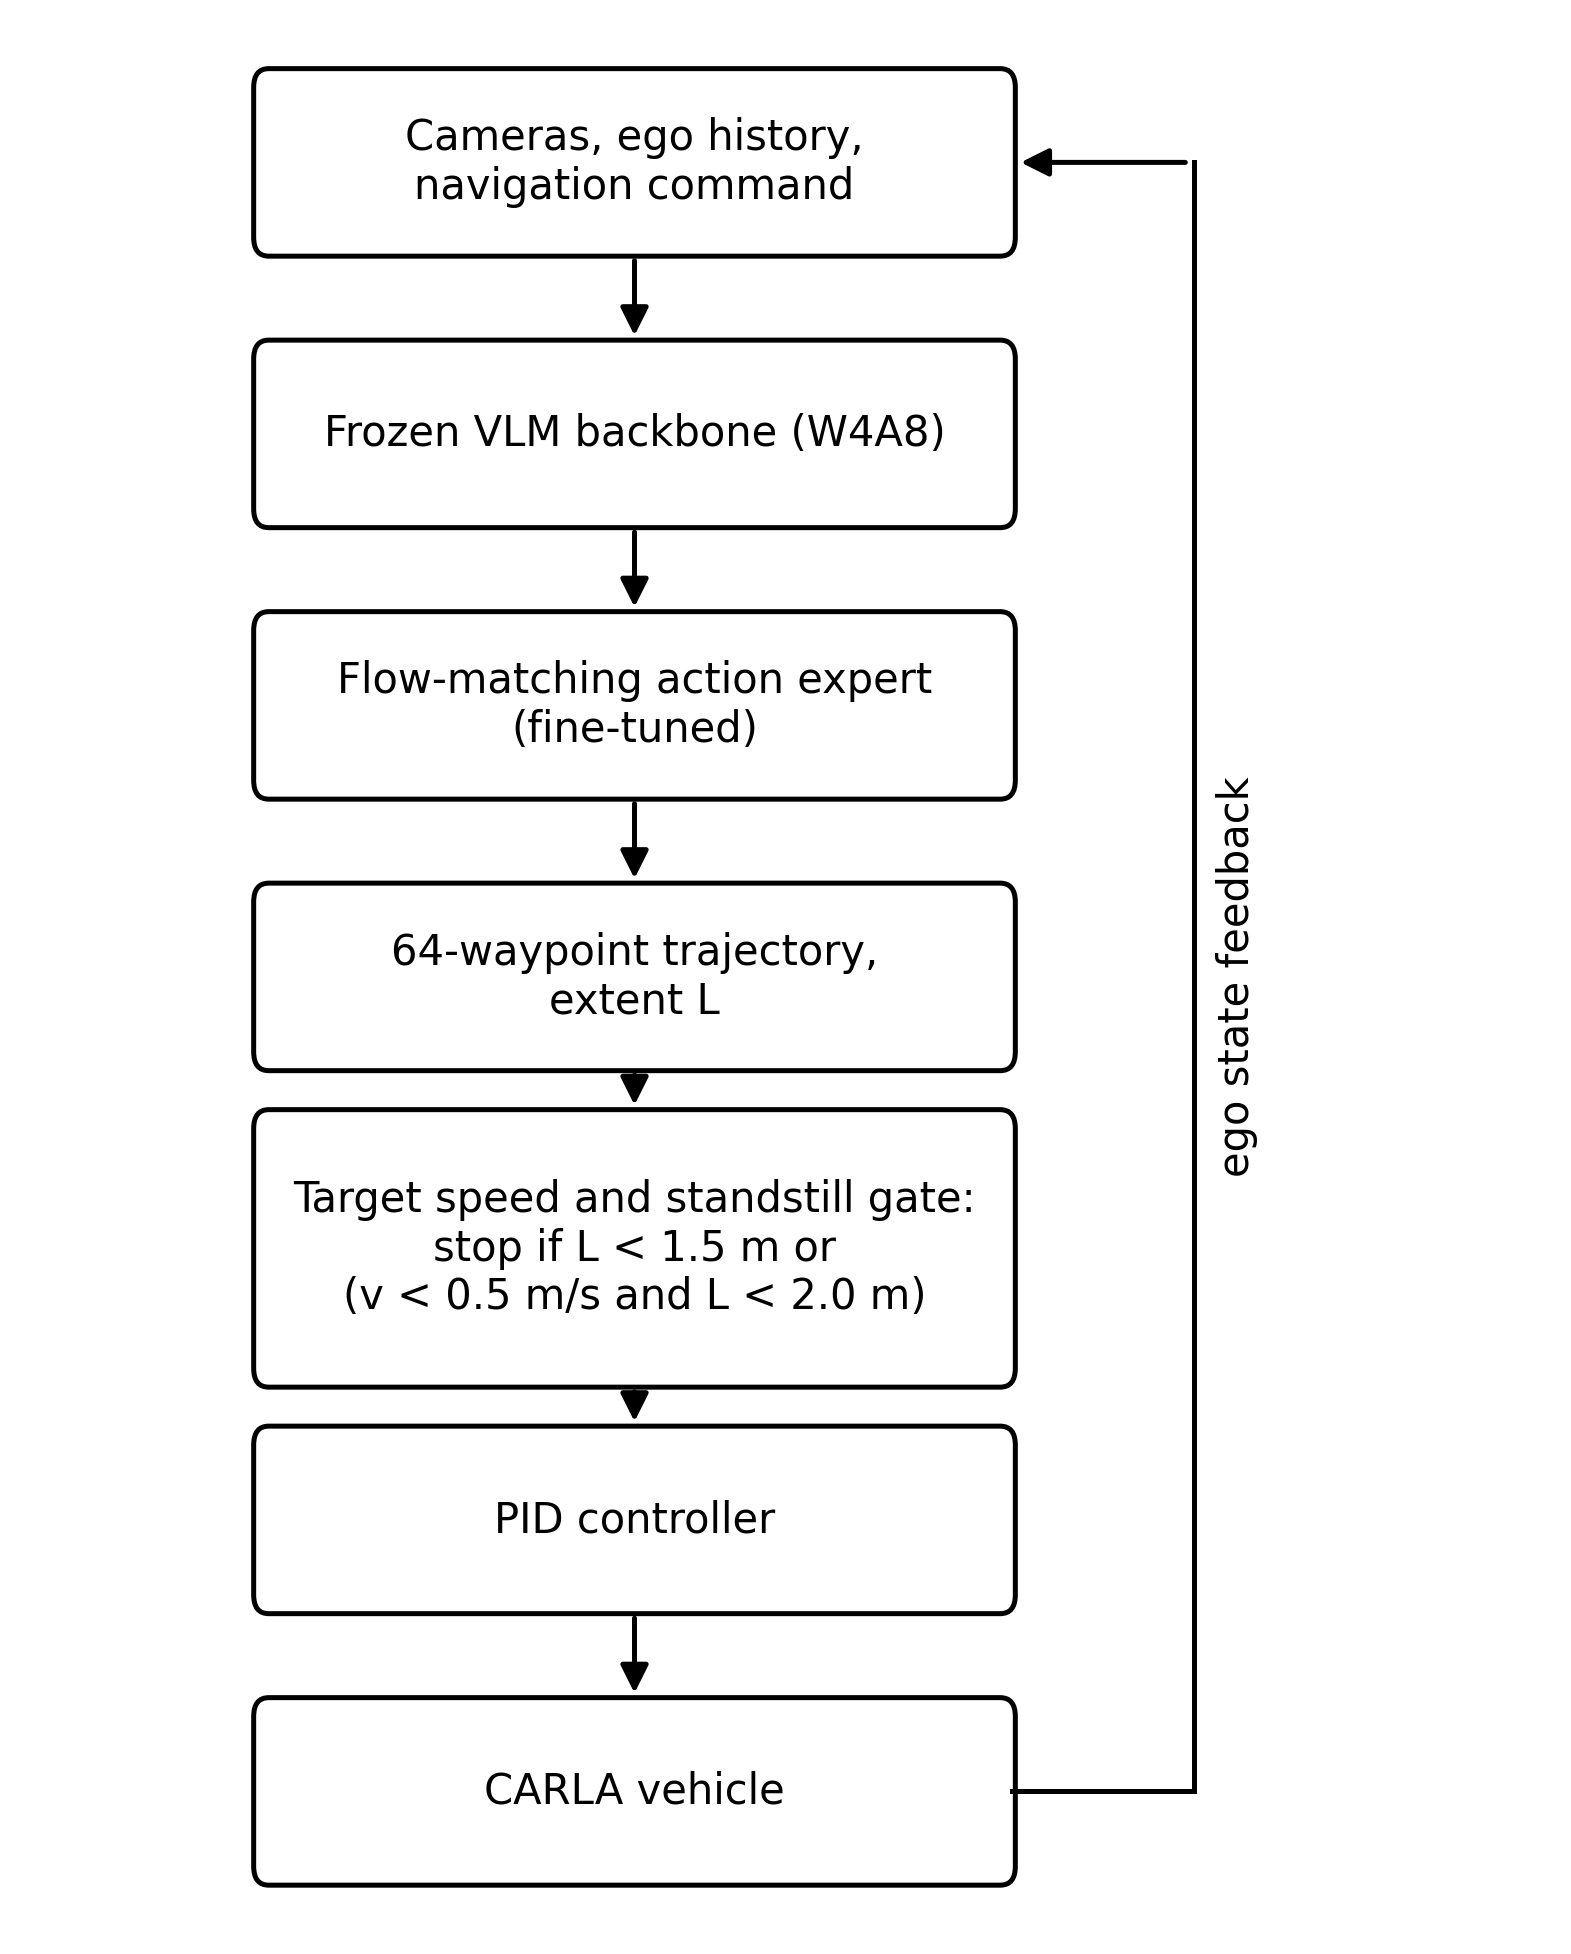
\includegraphics[width=\linewidth,height=0.8\textheight,keepaspectratio]{figure_1.png}
\caption{Inference and control pipeline in closed loop: camera images, ego history and navigation command; frozen VLM backbone; fine-tuned flow-matching action expert; 64-waypoint trajectory with extent L; target speed and standstill gate; PID controller; CARLA vehicle, with ego-state feedback. W4A8 denotes quantization to 4-bit weights and 8-bit activations.}
\end{figure}

\section{Experimental Results}

\subsection{Evaluation Protocol and Disclosures}

Routes and simulator. We use 44 Bench2Drive routes, one per scenario type. With a 10B-parameter policy one route takes about 22 minutes on an RTX 4090, which is why the full 220-route suite was not run for every model. Because of this subset and the custom controller, the Driving Scores reported here are not comparable with published 220-route Bench2Drive results. Evaluation ran in CARLA 0.9.15, in synchronous mode at 20 Hz and at rendering quality Low.

Runs and stages. Every fine-tuned checkpoint was served by the full-loading server of Section 3.4. The tests of the 6,400-sample pair were committed before the first route of the evaluation was run (ANALYSIS\_ADDENDUM \S{}25; dates in Supplementary Section S4.1). The evaluation had two stages: a first pass of the two 6,400-sample checkpoints (Section 4.3), and a second stage that was to follow if the plan-level test of the first stage was met and was otherwise to be decided anew. That test was met. The second stage comprises the second pass of both checkpoints, the run without the gate, the decoupling checkpoint, the 1,600-sample pair and the history-swap test (Sections 4.3 to 4.6 and 4.8). One server process served all routes of a job, and its streaming cache was not cleared between routes; this is the same for every checkpoint and pass.

Termination rule and censoring. The harness ends a route after 4,000 ticks (200 s) or after 1,200 consecutive ticks (60 s) with ego speed below 0.1 m/s. The standstill fraction is therefore censored: a model that stops for good accrues at most 60 s of final standstill. The unadapted policy was evaluated under the same rule. We call this run \texttt{Base\mbox{-}Rerun}, because a preliminary run of \texttt{Base} predates the rule, and every closed-loop comparison with the unadapted policy uses it.

Non-determinism. Every run used the same launcher and termination rule, and the same agent file except in the runs without the gate (Section 4.4) and in the history-swap test (Section 4.8). The model server does not seed its noise draws, so two runs of the same checkpoint differ from the first step. Between the two passes of each 6,400-sample checkpoint the per-route standstill difference had a standard deviation of 24.73 pp (\texttt{Golden\mbox{-}6400}) and 18.29 pp (\texttt{Flooded\mbox{-}6400}), with intraclass correlations of 0.67 and 0.84 for standstill and 0.70 and 0.68 for Driving Score (post hoc). Per-route comparisons and small strata are therefore descriptive only.

Collisions. The leaderboard merges repeated contacts with the same actor before logging, so logged collisions are not per-tick counts. We additionally merge, within each route, entries with the same actor identifier and report these as collision events.

Pre-specification. The rules referred to in this paper are files in the project repository with commit times in that repository; they were not time-stamped by a third party. (i) The tests of the first pass (F1, F2) and the repeat rule for the second pass (R1 to R3) were committed before the first route of the evaluation was run (Section 4.3). The checkpoints, the routes and the measures had been used in preliminary evaluations before that, so these are pre-specified tests on new runs, not a registration prior to all data. (ii) The rule of the same-input replay was committed before any inference of the replay (Section 4.2), the readings of the decoupling checkpoint before that checkpoint had run any route (Section 4.5), the reading of the run without the gate before that run (Section 4.4), and the rules of the history-swap test before any run of that test (Section 4.8). Each of these four analyses had been run once in the preliminary evaluations, and its outcome was known before the runs reported in this paper; the rules were not changed. (iii) The tests of the 1,600-sample pair (N1 to N3) were committed after \texttt{Golden\mbox{-}1600} had finished and while \texttt{Flooded\mbox{-}1600} was running, before any value of either run was computed (Section 4.6). (iv) All other analyses are post hoc or exploratory and are labelled as such. No decision rule was changed after any look at incomplete data. Supplementary Section S4.1 states for each when it was written down relative to its values, and gives the rerun rule with the launches that were repeated.

Statistics. Route-level differences are paired over the 44 routes; where a measure is defined on fewer routes, the number is given. The ratio of collision events per distance driven has a percentile bootstrap interval over routes. Tests are two-sided Wilcoxon signed-rank tests, and intervals are two-sided 95 \% BCa bootstrap intervals (20,000 resamples, seed 0). Absolute differences in percentages are given in percentage points (pp). Holm adjustment is made over the two tests named with each rule (Sections 4.3 and 4.6). All other p-values are unadjusted. The quantity estimated by each contrast is the mean paired difference over the routes; the interval is for this mean, whereas the Wilcoxon test is a rank test, so the two can disagree, and we say so where they do. For blocked time, which is zero on most routes, we also give an exact sign-flip permutation test of the mean difference. Each condition is one trained checkpoint (seed 42), so every test compares two specific checkpoints across routes and says nothing about variation between training runs.

Measures. Table 2 defines the measures used in this paper.

\begin{table}[htbp]
\small
\caption{The measures used in this paper: what each counts, at which level, and where it is defined.}
\begin{tabularx}{\linewidth}{>{\raggedright\arraybackslash}X>{\raggedright\arraybackslash}Xll}
\toprule
\textbf{Measure} & \textbf{Definition} & \textbf{Level} & \textbf{Defined in} \\
\midrule
Plan extent $L$ & Planar path length of the 64 predicted waypoints, from the first to the last; integrated from the current speed & Plan & \S{}3.1 \\
Near-stationary plan & $L < 1.5$ m (the gate's first clause); share of all logged steps (tests F1, R1 and N1) & Plan & \S{}4.3 \\
Stay-put plan & $L < 0.64$ m, a planned mean speed below 0.1 m/s; at \ensuremath{\leq} 0.5 m/s or at rest (\ensuremath{<} 0.1 m/s) & Plan & \S{}3.2, \S{}4.2 \\
Standstill time & Share of logged 20 Hz steps with speed \ensuremath{<} 0.1 m/s (tests F2 and N2) & Motion & \S{}4.1 \\
Crawling & Share of steps with 0.1 \ensuremath{\leq} speed \ensuremath{<} 1.0 m/s & Motion & \S{}4.3 \\
Blocked time & Standstill steps in a run of at least 100 consecutive steps (5 s) with throttle \ensuremath{\geq} 0.35 and no brake (test R3); 0.35 is the starting-torque floor of \S{}3.4, which applies only to plans of 2.5 m or more & Command & \S{}4.3 \\
Standstill outside blocked time & Standstill steps that are not in a blocked run (test R2) & Motion and command & \S{}4.3 \\
Gate condition & $L < 1.5$ m, or speed \ensuremath{<} 0.5 m/s and $L < 2.0$ m; sets target speed to zero and brakes & Controller & \S{}3.4 \\
Collision event & Leaderboard collision records merged by actor & Outcome & \S{}4.1 \\
Driving Score, route completion & Leaderboard scores per route & Outcome & \cite{ref3} \\
Success Rate & Share of routes completed without an infraction other than a minimum-speed record (Bench2Drive definition) & Outcome, descriptive & \S{}4.3 \\
Driving Efficiency & Ego speed as a percentage of the speed of the surrounding traffic, at 20 checkpoints per route; definition of the Bench2Drive tool \cite{ref3} (test N3) & Outcome & \S{}4.3 \\
\bottomrule
\end{tabularx}
\end{table}

\subsection{Same-Input Replay}

Closed-loop rates of plans are taken in the states each model reached, so they do not compare the experts on the same inputs. To make that comparison we replayed recorded states through the engine of the model server, one expert per process. The states are the 384 samples of the shared validation split with a speed of 0.5 m/s or less (67 clips from 31 source logs); the split is held out by route from every training set. For each state the engine received the frame window 0.1 s earlier and then the window of the state itself, as in streaming deployment, on a fresh stream, and returned 16 sampled plans. The random seed was fixed per state and was the same for every expert. The outcome is the stay-put share, the share of the 16 plans with $L < 0.64$ m. States of one source log are dependent, so the share is averaged within each log and the experts are compared over the 31 logs with the paired statistics of Section 4.1. The comparison was committed before any inference of the replay (ANALYSIS\_ADDENDUM \S{}21). The statistic reported here and its reading were fixed before any of the runs of this section (\S{}24), with the outcome of a preliminary replay known. In the demonstrations the future stays put in 15 of the 384 states (3.91 \%).

Do the experts differ on identical inputs? They do. \texttt{Golden\mbox{-}6400} had a stay-put share of 0.35 \% and \texttt{Flooded\mbox{-}6400} of 17.61 \%, as means over the 31 source logs (\textbf{\ensuremath{-}17.26 pp}, CI [\ensuremath{-}23.78, \ensuremath{-}12.13], p = $5.6 \times 10^{-6}$); the share of \texttt{Golden\mbox{-}6400} was lower in 27 logs, higher in none and equal in 4. Pooled over the 384 states the shares are 0.63 \% and 22.71 \% (difference 22.07 pp); the values above are means over the 31 source logs, which are the unit of the test. By the rule fixed in advance, the two experts differ on identical inputs. The direction is that of the closed-loop shares. Pooled over all plans, \texttt{Flooded\mbox{-}6400} returned a plan that starts ($L \ge 2.0$ m) in 50.18 \% of plans and \texttt{Golden\mbox{-}6400} in 92.79 \%.

In which direction did fine-tuning move the policy? In both, in these two checkpoints (descriptive). \texttt{Base} returned stay-put plans in 3.28 \%. Against it, \texttt{Golden\mbox{-}6400} was lower (\ensuremath{-}2.92 pp, CI [\ensuremath{-}4.60, \ensuremath{-}1.95]) and \texttt{Flooded\mbox{-}6400} higher (+14.33 pp, CI [9.46, 20.62]). On these states, the one training run on the balanced mix therefore lowered the stay-put share of the base model and the one on the obstacle-heavy mix raised it; with one run per mix this shows the direction of each checkpoint and not an effect of the mix. The decoupling checkpoint was at 0.99 \%: far below \texttt{Flooded\mbox{-}6400} (\ensuremath{-}16.62 pp, CI [\ensuremath{-}22.78, \ensuremath{-}11.74]) and slightly above \texttt{Golden\mbox{-}6400} (+0.63 pp, CI [0.24, 1.44]). The 1,600-sample pair differed in the same direction and by less: 2.59 \% for \texttt{Golden\mbox{-}1600} against 5.34 \% for \texttt{Flooded\mbox{-}1600} (\ensuremath{-}2.75 pp, CI [\ensuremath{-}4.71, \ensuremath{-}1.53]); Section 4.6 gives this pair in closed loop.

What do the plans look like on a single state? Figure 2 shows the 16 plans of the three 6,400-sample checkpoints on two of the replayed states. It is an illustration; no test is attached to it. The two states were chosen by a rule fixed before any state was looked at (ANALYSIS\_ADDENDUM \S{}27). For each state, $d$ is the number of stay-put plans of \texttt{Flooded\mbox{-}6400} minus that of \texttt{Golden\mbox{-}6400}, out of 16. Panel (a) is the state whose $d$ is closest to the mean over the 384 states (mean 3.53; $d = 4$), a signalized junction at which the vehicle stands. There \texttt{Flooded\mbox{-}6400} returned 4 stay-put plans and a median extent of 1.08 m, and the other two checkpoints returned no stay-put plan and median extents of 5.47 m and 5.44 m. Panel (b) is the state with the largest $d$ of the set ($d = 16$), a pedestrian crossing at night. All 16 plans of \texttt{Flooded\mbox{-}6400} stayed put, none of \texttt{Golden\mbox{-}6400} did, although its median extent of 1.41 m is below the 1.5 m at which the standstill gate holds the vehicle, and 8 of \texttt{Decoupling\mbox{-}6400} did. At a pedestrian crossing staying put may be the required behaviour, and for neither state do we know which plan is right; the demonstrated futures are not shown. The figure shows how far the checkpoints can differ on one input and nothing more, and panel (b) is the extreme of the set, not a typical state.

\begin{figure}[htbp]
\centering
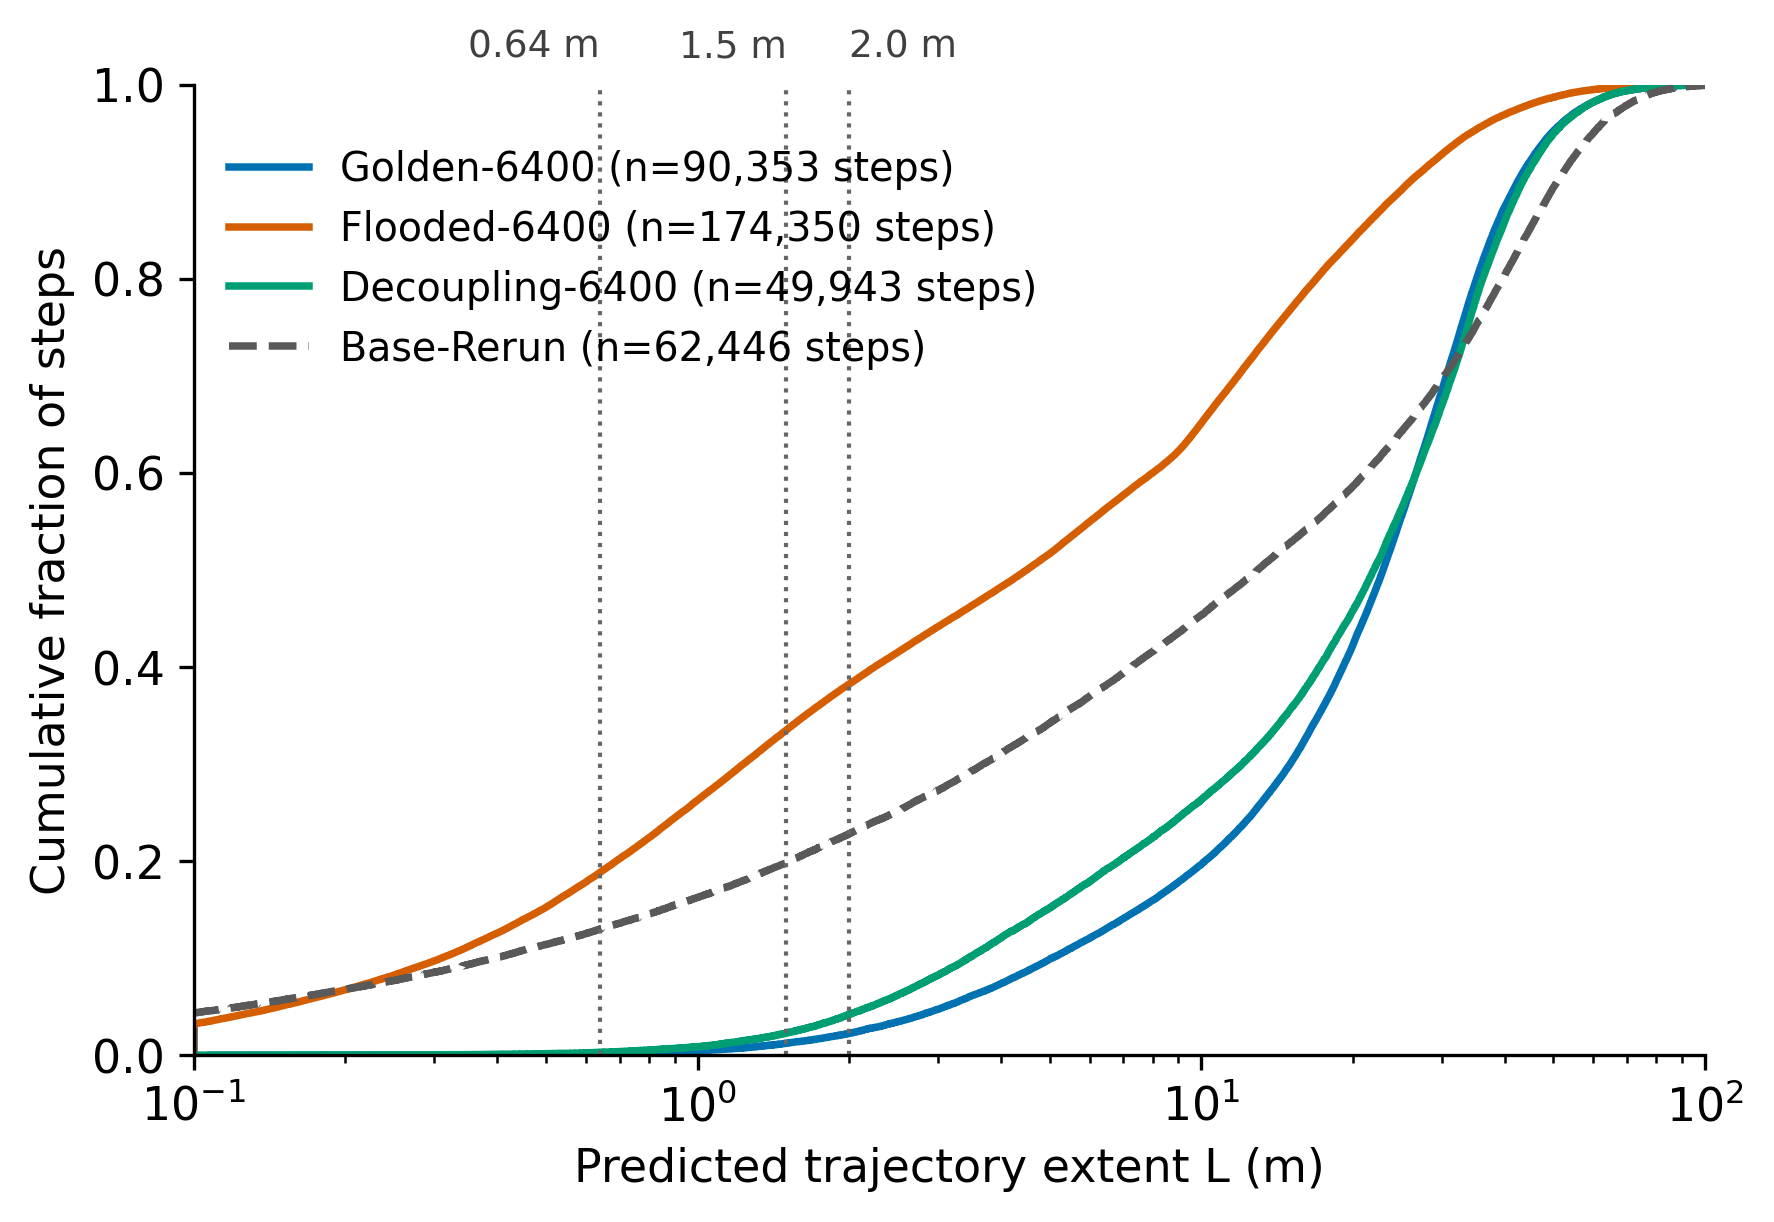
\includegraphics[width=\linewidth,height=0.8\textheight,keepaspectratio]{figure_2.png}
\caption{Sampled plans on two replayed states (illustrative). Left: front camera frame of the state with its scenario type, speed and navigation command; the night frame of panel (b) is brightened for print. Right: extent L of the 16 plans sampled by Golden-6400, Flooded-6400 and Decoupling-6400 on that state, sorted by L. Open markers are stay-put plans (L \ensuremath{<} 0.64 m, dotted line); the dashed line is the 1.5 m threshold of a near-stationary plan. Panel (a) is the state closest to the mean difference in stay-put plans between Flooded-6400 and Golden-6400 and panel (b) the state with the largest difference; both follow a rule fixed in advance. The vertical scales of the two panels differ. The planned paths are nearly straight (lateral displacement below 0.15 m), so extents are shown and not paths. The plans were computed again for this figure in new processes with the replay code and seeds unchanged, and on these two states their extents agree with the stored ones.}
\end{figure}

Is the replay reproducible? Within a process it is; between processes, not fully. No state failed for any expert. At the end of each process the first three states were run again with the same seeds, and the plans were reproduced exactly, so the output is reproducible within a process. It was not fully reproducible between processes. A second process of the unchanged base model, with the same code and seeds, differed from the first in rationale text and plans in 8 of the 24 states compared, and a later process of the base model had a stay-put share of 4.23 \% against 3.28 \% for the first. We do not know the cause. The comparisons of this section therefore carry an uncertainty of about 1 pp from this source, estimated from one pair of processes of one model. It is small against the difference between the two 6,400-sample checkpoints and is not small against the smaller contrasts above (+0.63 pp between \texttt{Decoupling\mbox{-}6400} and \texttt{Golden\mbox{-}6400}, \ensuremath{-}2.75 pp for the 1,600-sample pair), which we therefore report without relying on them. The contrast between \texttt{Golden\mbox{-}6400} and \texttt{Base} holds against the later base process as well (\ensuremath{-}3.88 pp, CI [\ensuremath{-}5.74, \ensuremath{-}2.59]). The plans computed again for Figure 2, in new processes of the three fine-tuned checkpoints, agreed with the stored ones on both states.

What does the replay not show? The states are those a privileged expert driver reached; states after a collision, and other states that only the learned policies reach, are absent. Each state is one prefill and one streaming step, not a long stream. The replay shows that the experts differ on the same inputs. It does not show why, and with one training run per mix it cannot attribute the difference to the data mix.

\subsection{The Matched Pair at 6,400 Samples}

Protocol. The two 6,400-sample checkpoints were evaluated on the 44 routes. The agent file, the default controller, the launcher, the termination rule and the rerun rule (a route without a score is launched again, up to three launches; a scored route is never relaunched) were fixed before the runs. A route counted only if the full-loading server (Section 3.4), with a clean loading report, served it from start to end. All 44 routes of both checkpoints were scored and counted. One route of \texttt{Flooded\mbox{-}6400} ended without a score at its first launch and was launched again under the rerun rule; no route was scored twice. The second pass of both checkpoints followed under the same protocol. All 44 routes of both checkpoints were again scored and counted, and one route of \texttt{Golden\mbox{-}6400} was launched a second time under the rerun rule.

Tests fixed before the runs. F1, the primary test, is the share of logged steps with a near-stationary plan ($L < 1.5$ m), \texttt{Golden\mbox{-}6400} minus \texttt{Flooded\mbox{-}6400}, paired by route. It is met if the difference is negative, the interval lies below zero and p \ensuremath{<} 0.05. F2 is the standstill time, read by cases fixed in advance: an interval below zero with a point estimate of \ensuremath{-}4.0 pp or lower counts as a strong result. Both use the statistics of Section 4.1 and are reported with Holm-adjusted p-values over the two. All other comparisons in this section are descriptive. The repeat rule for the second pass was fixed at the same time. On the second pass alone, R1 is the share of near-stationary plans, R2 the standstill outside blocked time and R3 the blocked time. Each counts as replicated if its difference has the sign of the first pass, its interval excludes zero and p \ensuremath{<} 0.05, with Holm adjustment over R2 and R3.

Does the balanced checkpoint return near-stationary plans less often? It does, by a wide margin (Table 3; Figure 3 shows both passes pooled). \texttt{Golden\mbox{-}6400} returned a near-stationary plan in 1.31 \% of steps and \texttt{Flooded\mbox{-}6400} in 26.80 \%, a difference of \textbf{\ensuremath{-}25.49 pp} (CI [\ensuremath{-}31.69, \ensuremath{-}19.63], p = $1.1 \times 10^{-13}$, Holm $2.3 \times 10^{-13}$; \textbf{F1 is met}). Among the steps at 0.5 m/s or less the difference was of the same size: \texttt{Golden\mbox{-}6400} returned a stay-put plan in 1.06 \% of these steps and \texttt{Flooded\mbox{-}6400} in 26.44 \% (\ensuremath{-}25.38 pp, CI [\ensuremath{-}29.82, \ensuremath{-}21.44]; 35 routes), and a plan that starts in 89.31 \% against 43.47 \%. These closed-loop shares agree in direction with the shares of Section 4.2, which were measured on identical inputs.

\begin{table}[htbp]
\small
\caption{\texttt{Golden\mbox{-}6400} / \texttt{Flooded\mbox{-}6400} on 44 routes with the default controller, first pass. Mean of per-route values, with the paired difference and its 95 \% BCa interval in parentheses. F1 and F2 were specified before the runs; all other rows are descriptive. For reference, the unadapted policy (\texttt{Base\mbox{-}Rerun}, one pass) had near-stationary plans in 13.24 \% of steps and a standstill time of 36.28 \%. The three plan rows at 0.5 m/s or less use the 35 routes with at least 20 such steps in both arms.}
\begin{tabularx}{\linewidth}{>{\raggedright\arraybackslash}X>{\raggedright\arraybackslash}X}
\toprule
\textbf{Measure (\% of steps unless stated)} & \textbf{\texttt{Golden\mbox{-}6400} / \texttt{Flooded\mbox{-}6400} (difference; 95 \% CI)} \\
\midrule
Near-stationary plans, $L < 1.5$ m, all steps (F1) & 1.31 / 26.80 (\ensuremath{-}25.49; [\ensuremath{-}31.69, \ensuremath{-}19.63]) \\
Stay-put plans, $L < 0.64$ m, at \ensuremath{\leq} 0.5 m/s & 1.06 / 26.44 (\ensuremath{-}25.38; [\ensuremath{-}29.82, \ensuremath{-}21.44]) \\
Stay-put plans at rest (\ensuremath{<} 0.1 m/s) & 1.18 / 29.09 (\ensuremath{-}27.91; [\ensuremath{-}32.14, \ensuremath{-}24.02]) \\
Plans that start, $L \ge 2.0$ m, at \ensuremath{\leq} 0.5 m/s & 89.31 / 43.47 (45.83; [40.32, 51.38]) \\
Total standstill time (F2) & 22.97 / 46.66 (\ensuremath{-}23.69; [\ensuremath{-}33.48, \ensuremath{-}15.08]) \\
Standstill outside blocked time & 10.28 / 46.66 (\ensuremath{-}36.38; [\ensuremath{-}45.55, \ensuremath{-}28.16]) \\
Blocked time & 12.69 / 0.00 (12.69; [6.10, 22.48]) \\
Time at crawling speed (0.1 to 1.0 m/s) & 6.81 / 12.27 (\ensuremath{-}5.46; [\ensuremath{-}8.58, \ensuremath{-}2.90]) \\
Driving Score (points) & 54.02 / 43.51 (10.52; [2.59, 19.09]) \\
Route completion (\%) & 71.55 / 63.19 (8.36; [1.76, 16.29]) \\
Collision events per route & 0.64 / 0.64 (0.00; [\ensuremath{-}0.34, 0.23]) \\
Mean speed (m/s) & 2.17 / 0.96 (1.21; [0.97, 1.45]) \\
\bottomrule
\end{tabularx}
\end{table}

\begin{figure}[htbp]
\centering
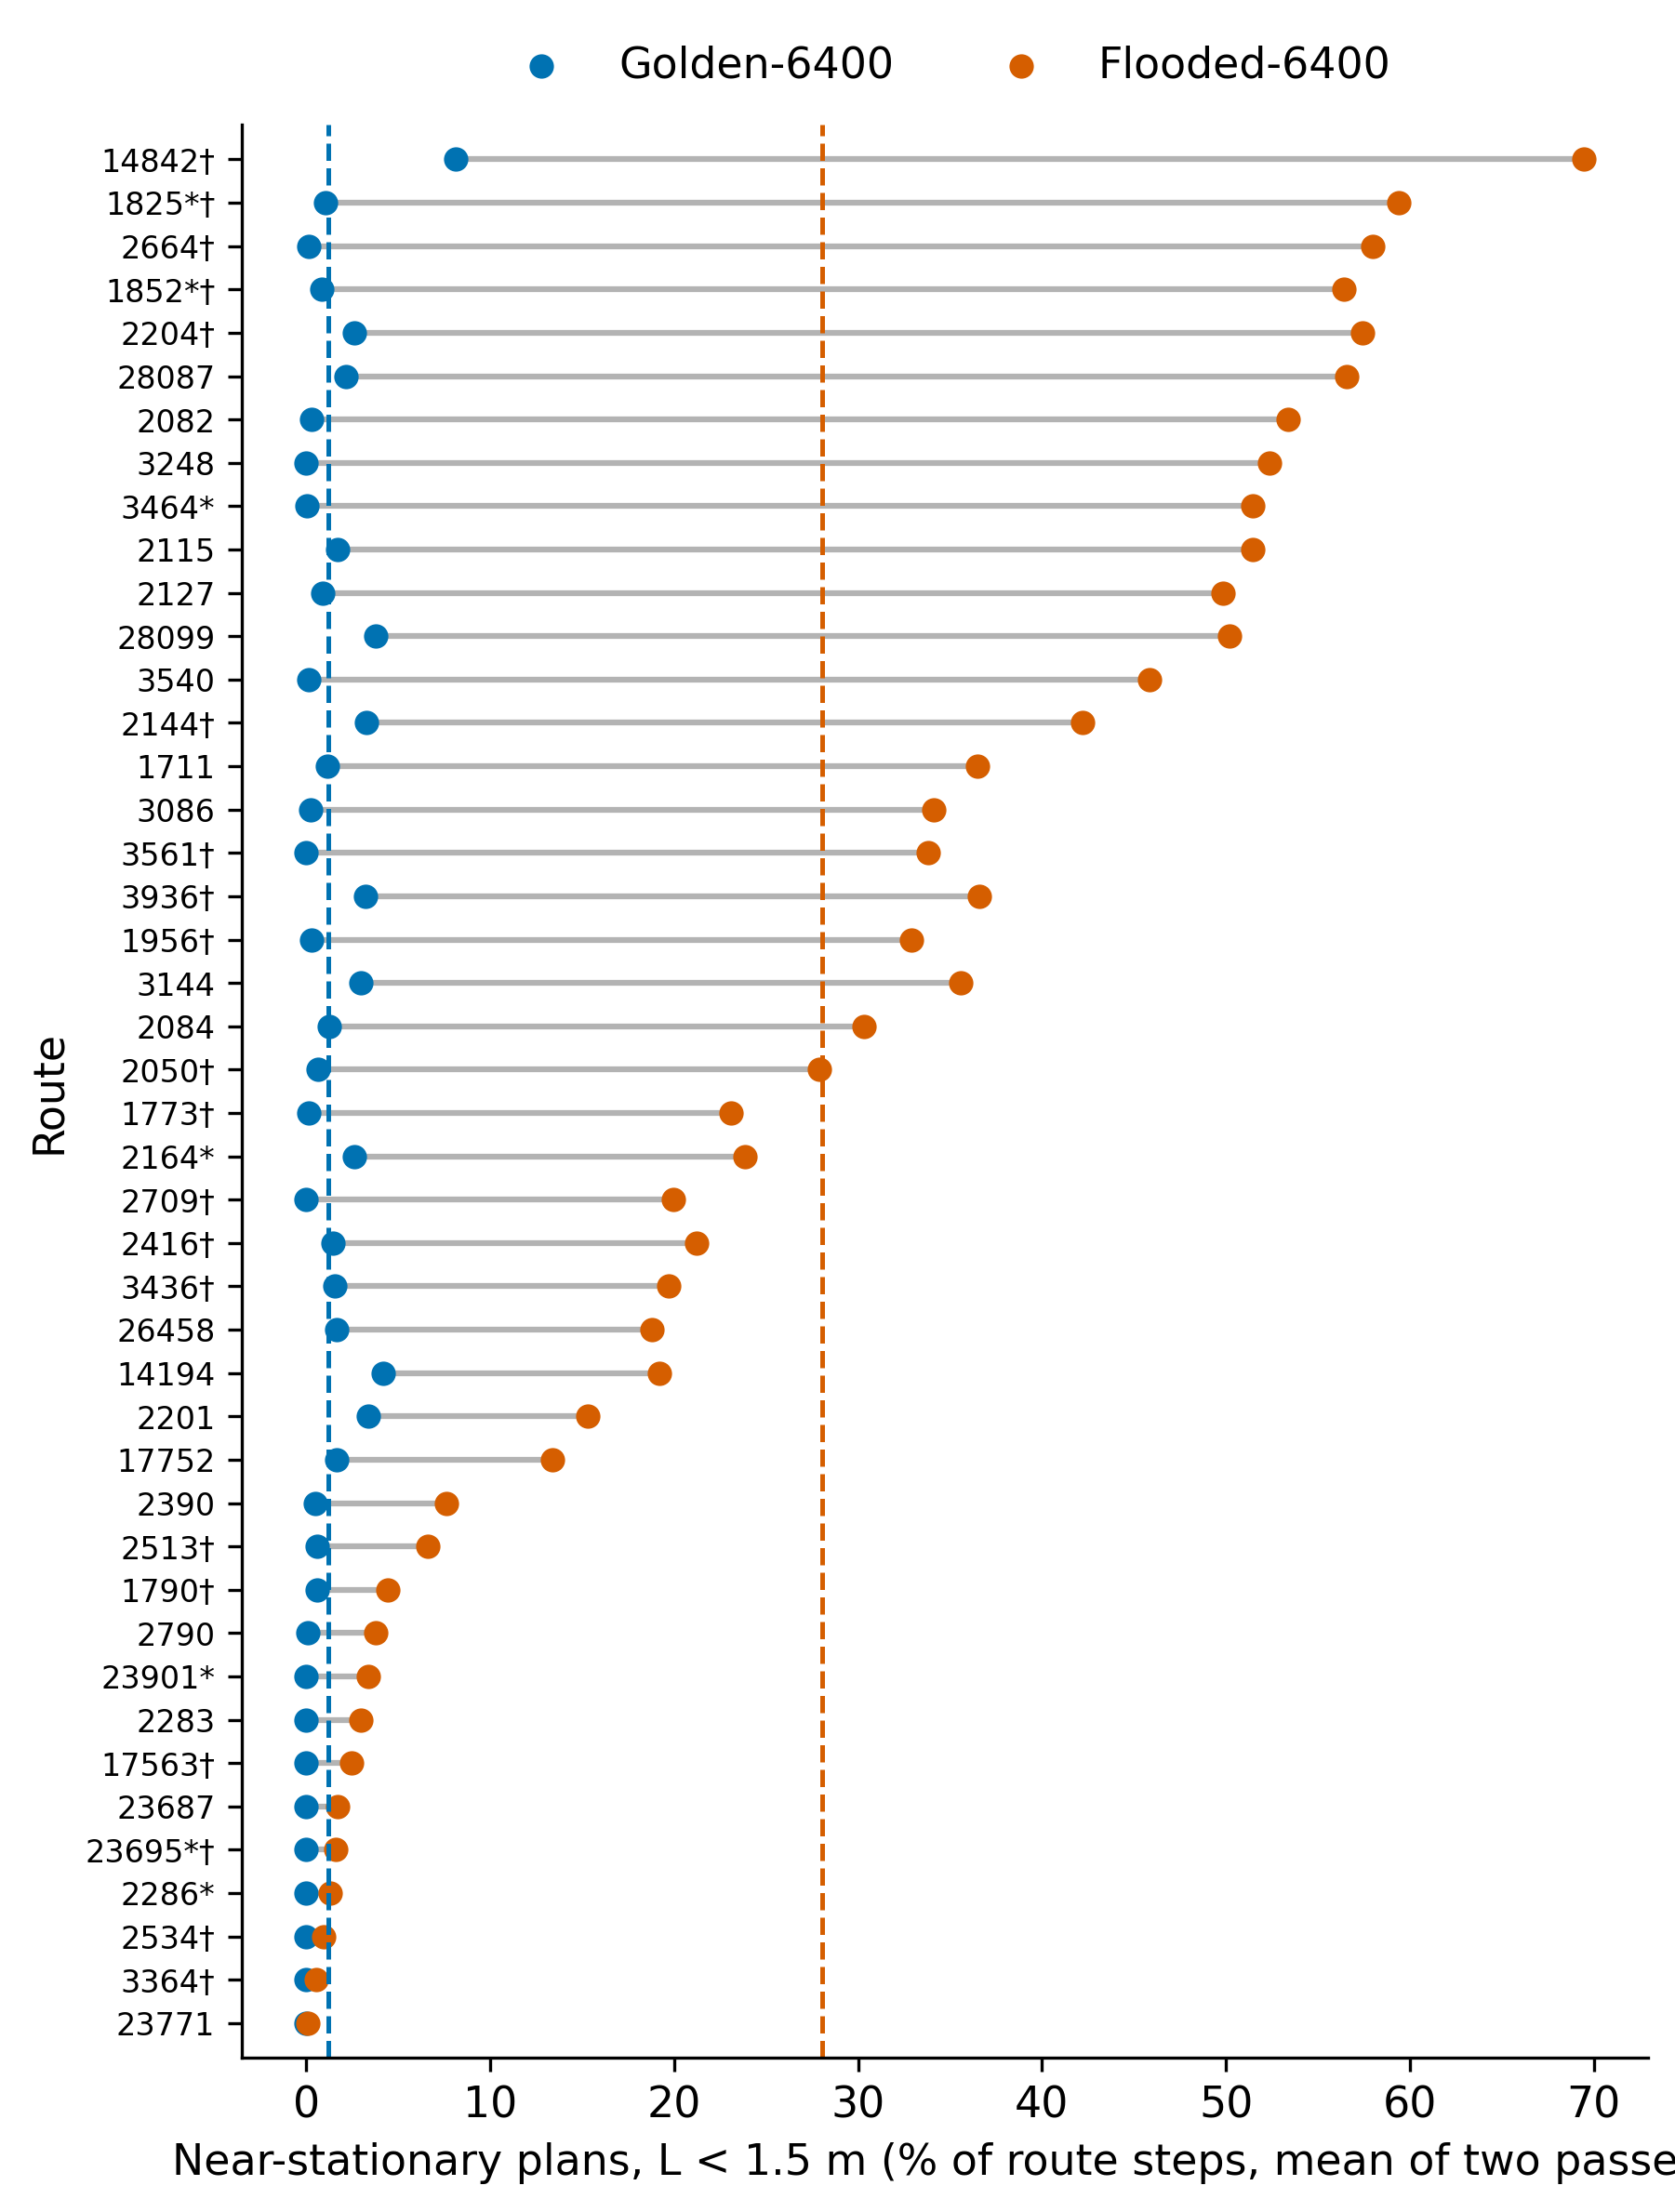
\includegraphics[width=\linewidth,height=0.8\textheight,keepaspectratio]{figure_3.png}
\caption{Empirical cumulative distribution of the predicted trajectory extent L over all logged steps of the 44 routes: Golden-6400 and Flooded-6400 (both passes pooled), Decoupling-6400 and the unadapted policy (Base-Rerun; one pass each). Logarithmic axis; values below 0.1 m are shown at 0.1 m. Dotted lines mark 0.64, 1.5 and 2.0 m. The curves pool the steps of all routes, so their values at 1.5 m differ from the means of per-route shares given in the text (28.04 \% and 13.24 \%), in which every route has the same weight.}
\end{figure}

Does the vehicle stand still less? It does. \texttt{Golden\mbox{-}6400} stood still for 22.97 \% of the route time and \texttt{Flooded\mbox{-}6400} for 46.66 \%, a difference of \textbf{\ensuremath{-}23.69 pp} (CI [\ensuremath{-}33.48, \ensuremath{-}15.08], p = $3.3 \times 10^{-6}$, Holm $3.3 \times 10^{-6}$; \textbf{F2 is a strong result} by the rule fixed in advance). \texttt{Flooded\mbox{-}6400} also spent more time crawling (difference \ensuremath{-}5.46 pp, CI [\ensuremath{-}8.58, \ensuremath{-}2.90]) and drove at less than half the mean speed (0.96 against 2.17 m/s), and the 60 s standstill rule ended 10 of its routes against 5 of \texttt{Golden\mbox{-}6400}.

Where does the remaining standstill come from? The two checkpoints stood still for different reasons. \texttt{Flooded\mbox{-}6400} had no blocked time on any route: none of its standstill was time in which the controller commanded acceleration for 5 s or more and the vehicle did not move. \texttt{Golden\mbox{-}6400} had blocked time on 10 routes (12.69 \% of steps on average; sign-flip permutation test p = 0.002). Outside blocked time, \texttt{Golden\mbox{-}6400} stood still for 10.28 \% of steps against 46.66 \% (\ensuremath{-}36.38 pp, CI [\ensuremath{-}45.55, \ensuremath{-}28.16]). The balanced checkpoint thus stood still far less, and part of the standstill it kept was time in which it was commanded to move and did not.

What is the vehicle doing while it is blocked? It keeps commanding forward motion, in most cases within 10 m of a recorded collision position (post hoc, descriptive). The plans at the blocked steps of \texttt{Golden\mbox{-}6400} were forward plans: 2.0 m or longer in 97.7 \% of them in the first pass and 99.7 \% in the second, with a median length of 11.8 m and 20.0 m. Of these steps, 91.4 \% and 100.0 \% lay within 10 m of a recorded collision position. The episodes lay mostly at another vehicle, in scenarios with an obstacle in the lane (an opening door, an accident, a parked or construction obstacle, a lead vehicle braking hard) and at junction turns, and most of these routes were then ended by the harness with status TickRuntime (6 of 10 and 8 of 11), which covers the time limit and the 60 s standstill rule. On at least 3 and 6 of them the final blocked run itself lasted 60 s and triggered the standstill rule, so the harness cuts blocked time off at 60 s per run. The position match is weak evidence taken alone. Over the nine closed-loop runs of fine-tuned checkpoints, long stops that were not blocked also lay within 10 m of a recorded collision position in 91 of the 119 cases on a route with a collision record (76.5 \%). The match is thus not specific to blocked time, although it exceeds what the routes alone give: on the routes with a blocked run, 34.6 \% and 30.9 \% of the distance travelled lay within 10 m of such a position. The records give neither the order of contact and stop nor the duration of contact. Blocked time is therefore co-located with recorded collisions, and whether it adds harm beyond the recorded contact cannot be measured from these logs. Supplementary Table S2 gives the collision events of both checkpoints on the routes with blocked time (post hoc). On these routes \texttt{Golden\mbox{-}6400} had 14 events against 8 for \texttt{Flooded\mbox{-}6400} in the first pass (10 routes) and 15 against 5 in the second (11 routes); on the remaining routes it had 14 against 20 and 21 against 10. What the plans do show is that blocked time is not a second form of staying put: the model asks for motion, so a controller rule that releases a held stop would not remove it.

Does the difference recur in a second pass? It does, on all three measures of the repeat rule (Table 4; Figure 4 shows the per-route mean of the two passes for near-stationary plans). In the second pass alone \texttt{Golden\mbox{-}6400} returned a near-stationary plan in 1.12 \% of steps and \texttt{Flooded\mbox{-}6400} in 29.28 \% (\ensuremath{-}28.16 pp, CI [\ensuremath{-}34.81, \ensuremath{-}21.75], p = $1.1 \times 10^{-13}$; \textbf{R1 replicated}). Its standstill outside blocked time was 9.15 \% against 48.44 \% (\ensuremath{-}39.29 pp, CI [\ensuremath{-}48.36, \ensuremath{-}30.34], Holm p = $3.1 \times 10^{-11}$; \textbf{R2 replicated}), and its blocked time 15.90 \% against 0.00 \% (+15.90 pp, CI [8.06, 26.85], Holm p = 0.0033; \textbf{R3 replicated}). The p-value of R3 is the normal approximation that the script of the rule returns when 33 of the 44 differences are zero; the exact sign-flip test over the 11 non-zero pairs gives p = 0.00098. With a run length of 40 or 200 steps, or with a throttle threshold of 0.2, in the definition of blocked time the second-pass difference was +16.81, +15.49 and +16.24 pp, each with an interval above zero. The standstill outside blocked time differed by \ensuremath{-}40.20, \ensuremath{-}38.88 and \ensuremath{-}39.63 pp under the same three settings, each with an interval below zero. \texttt{Flooded\mbox{-}6400} again had no blocked time on any route, and \texttt{Golden\mbox{-}6400} had it on 11. Total standstill time differed by \ensuremath{-}23.39 pp in the second pass (CI [\ensuremath{-}34.18, \ensuremath{-}12.11]) and by \ensuremath{-}23.54 pp over both passes (CI [\ensuremath{-}32.98, \ensuremath{-}14.89]). On the 37 routes without training overlap the three differences were of the same size (\ensuremath{-}28.25 pp, \ensuremath{-}39.43 pp and +12.71 pp, each with an interval that excludes zero). Between its two passes neither checkpoint changed detectably on any plan or standstill measure.

\begin{table}[htbp]
\small
\caption{\texttt{Golden\mbox{-}6400} / \texttt{Flooded\mbox{-}6400} on 44 routes with the default controller: first pass, second pass and the per-route mean of the two passes. Mean of per-route values, with the paired difference and its 95 \% BCa interval in parentheses. R1 to R3 are the measures of the repeat rule, which is decided on the second pass alone; all other entries are descriptive. \texttt{Base\mbox{-}Rerun} (one pass): near-stationary plans 13.24 \%, standstill time 36.28 \%, Driving Score 42.60.}
\begin{tabularx}{\linewidth}{>{\raggedright\arraybackslash}X>{\raggedright\arraybackslash}X>{\raggedright\arraybackslash}X>{\raggedright\arraybackslash}X}
\toprule
\textbf{Measure (\% of steps unless stated)} & \textbf{First pass} & \textbf{Second pass} & \textbf{Mean of the two passes} \\
\midrule
Near-stationary plans, $L < 1.5$ m, all steps (R1) & 1.31 / 26.80 (\ensuremath{-}25.49; [\ensuremath{-}31.69, \ensuremath{-}19.63]) & 1.12 / 29.28 (\ensuremath{-}28.16; [\ensuremath{-}34.81, \ensuremath{-}21.75]) & 1.22 / 28.04 (\ensuremath{-}26.83; [\ensuremath{-}32.83, \ensuremath{-}20.93]) \\
Standstill outside blocked time (R2) & 10.28 / 46.66 (\ensuremath{-}36.38; [\ensuremath{-}45.55, \ensuremath{-}28.16]) & 9.15 / 48.44 (\ensuremath{-}39.29; [\ensuremath{-}48.36, \ensuremath{-}30.34]) & 9.71 / 47.55 (\ensuremath{-}37.83; [\ensuremath{-}46.43, \ensuremath{-}29.76]) \\
Blocked time (R3) & 12.69 / 0.00 (12.69; [6.10, 22.48]) & 15.90 / 0.00 (15.90; [8.06, 26.85]) & 14.29 / 0.00 (14.29; [7.57, 24.21]) \\
Total standstill time & 22.97 / 46.66 (\ensuremath{-}23.69; [\ensuremath{-}33.48, \ensuremath{-}15.08]) & 25.05 / 48.44 (\ensuremath{-}23.39; [\ensuremath{-}34.18, \ensuremath{-}12.11]) & 24.01 / 47.55 (\ensuremath{-}23.54; [\ensuremath{-}32.98, \ensuremath{-}14.89]) \\
Time at crawling speed (0.1 to 1.0 m/s) & 6.81 / 12.27 (\ensuremath{-}5.46; [\ensuremath{-}8.58, \ensuremath{-}2.90]) & 6.61 / 10.71 (\ensuremath{-}4.10; [\ensuremath{-}6.32, \ensuremath{-}2.24]) & 6.71 / 11.49 (\ensuremath{-}4.78; [\ensuremath{-}7.02, \ensuremath{-}2.81]) \\
Driving Score (points) & 54.02 / 43.51 (10.52; [2.59, 19.09]) & 49.01 / 51.60 (\ensuremath{-}2.59; [\ensuremath{-}11.94, 6.51]) & 51.52 / 47.55 (3.96; [\ensuremath{-}3.06, 11.67]) \\
Route completion (\%) & 71.55 / 63.19 (8.36; [1.76, 16.29]) & 70.94 / 65.62 (5.32; [\ensuremath{-}1.67, 12.25]) & 71.24 / 64.40 (6.84; [0.80, 13.29]) \\
Collision events per route & 0.64 / 0.64 (0.00; [\ensuremath{-}0.34, 0.23]) & 0.82 / 0.34 (0.48; [0.23, 0.77]) & 0.73 / 0.49 (0.24; [0.00, 0.43]) \\
Mean speed (m/s) & 2.17 / 0.96 (1.21; [0.97, 1.45]) & 2.12 / 1.06 (1.06; [0.74, 1.36]) & 2.14 / 1.01 (1.13; [0.90, 1.38]) \\
\bottomrule
\end{tabularx}
\end{table}

\begin{figure}[htbp]
\centering
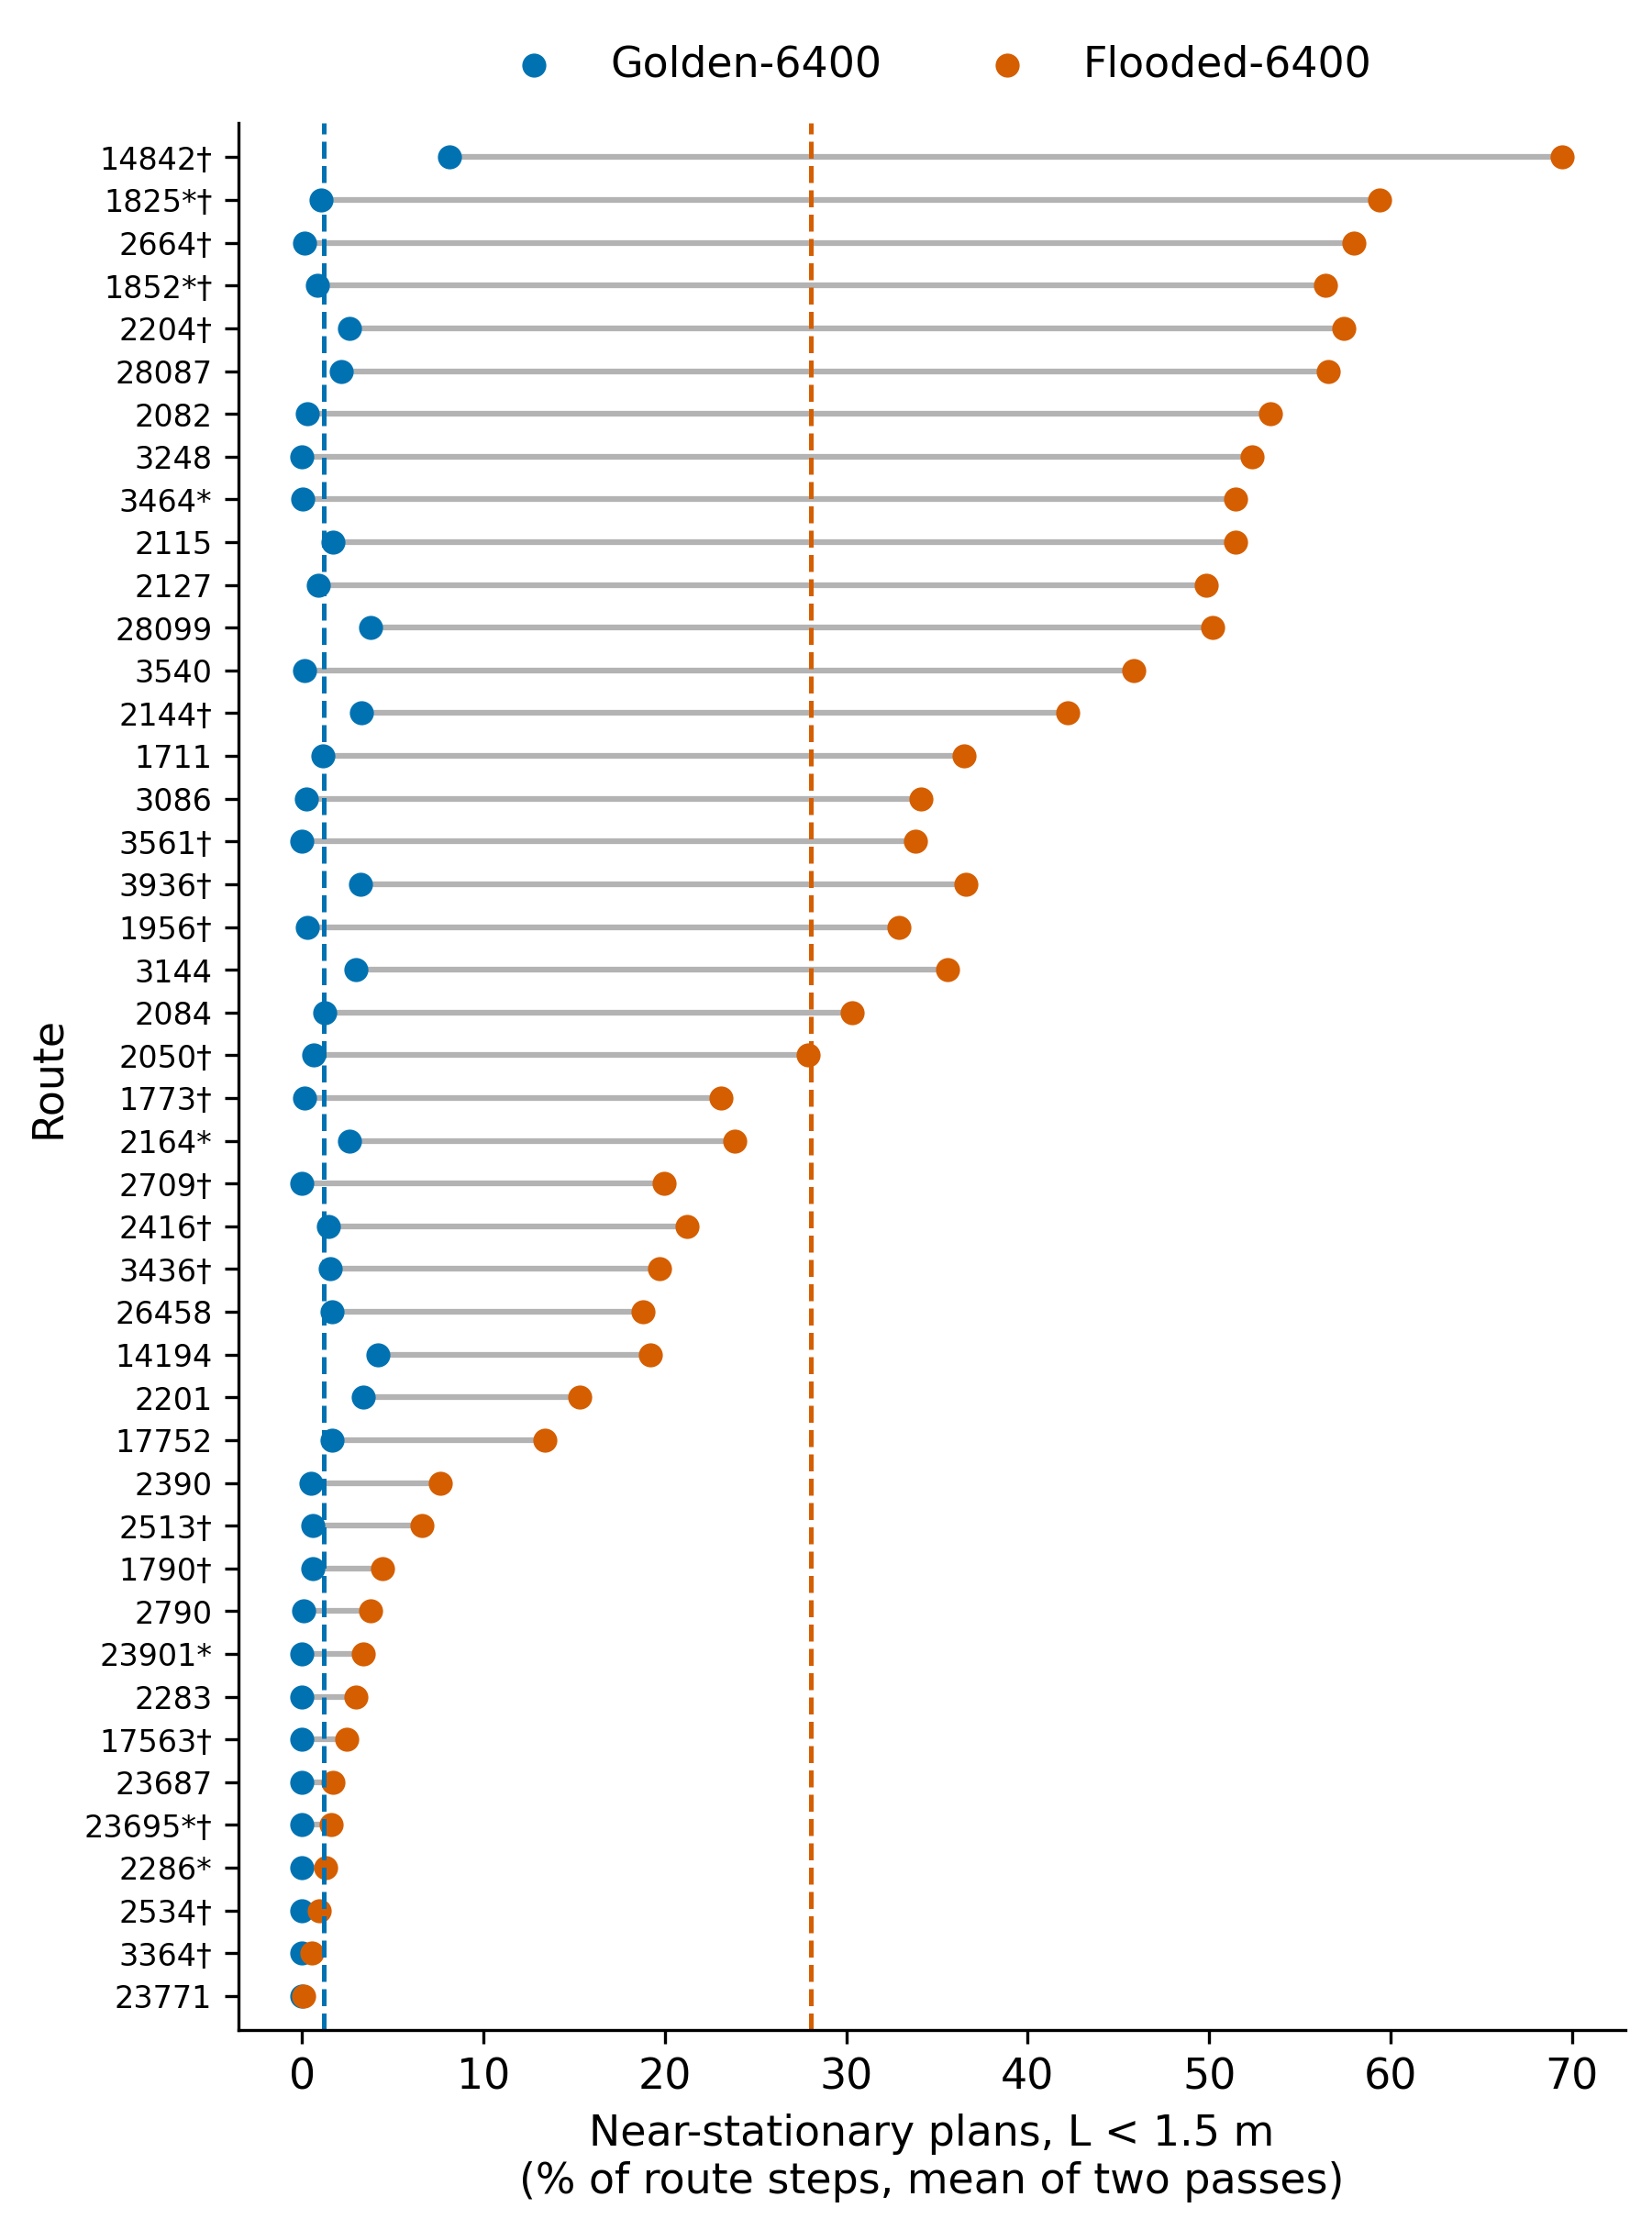
\includegraphics[width=\linewidth,height=0.8\textheight,keepaspectratio]{figure_4.png}
\caption{Share of steps with a near-stationary plan (L \ensuremath{<} 1.5 m) on each of the 44 routes for Golden-6400 and Flooded-6400 as the mean of the two passes, sorted by the paired difference. Dashed lines are the 44-route means. An asterisk marks the 7 routes touched by training samples and a dagger the 20 controller-tuning routes.}
\end{figure}

Does the balanced checkpoint score higher on the benchmark? Not detectably. In the first pass \texttt{Golden\mbox{-}6400} had the higher Driving Score, 54.02 against 43.51 (+10.52 points, CI [2.59, 19.09], p = 0.044). The outcome was not pre-specified, and it did not recur: in the second pass the scores were 49.01 against 51.60 (\ensuremath{-}2.59, CI [\ensuremath{-}11.94, 6.51]), and over both passes 51.52 against 47.55 (+3.96, CI [\ensuremath{-}3.06, 11.67], p = 0.36). Most of the change came from \texttt{Flooded\mbox{-}6400}, whose second pass scored 8.09 points above its first (CI [1.93, 15.16]) with 15 collision events against 28; no measure of \texttt{Golden\mbox{-}6400} differed detectably between its passes. Route completion was higher for \texttt{Golden\mbox{-}6400} over both passes, 71.24 \% against 64.40 \% (+6.84 pp, CI [0.80, 13.29], p = 0.0055); it completed 21 and 19 routes, and \texttt{Flooded\mbox{-}6400} 16 and 18. \texttt{Golden\mbox{-}6400} had 28 and 36 collision events and \texttt{Flooded\mbox{-}6400} 28 and 15, a difference of +0.24 events per route over both passes (CI [0.00, 0.43], p = 0.024). \texttt{Golden\mbox{-}6400} also drove farther. Per kilometre driven it had 8.07 events (64 in 7.93 km) and \texttt{Flooded\mbox{-}6400} 6.23 (43 in 6.90 km), a ratio of 1.29 whose interval includes one (CI [0.90, 1.92]). One pass of 44 routes was thus not enough to compare the two checkpoints on Driving Score or on collisions. The Bench2Drive Success Rate, the share of routes completed without an infraction other than a minimum-speed record, was 20.5 \% and 13.6 \% for \texttt{Golden\mbox{-}6400} in the two passes and 6.8 \% and 11.4 \% for \texttt{Flooded\mbox{-}6400} (+7.95 pp over both passes, CI [\ensuremath{-}2.27, 17.05]); \texttt{Base\mbox{-}Rerun} had 13.6 \%.

Is the balanced checkpoint faster? It is: about twice the progress per unit of route time and 1.6 times the speed while moving (post hoc, descriptive). On the 11 routes that both checkpoints completed in both passes, \texttt{Golden\mbox{-}6400} needed 45.62 s and \texttt{Flooded\mbox{-}6400} 76.51 s (\ensuremath{-}30.89 s, CI [\ensuremath{-}60.44, \ensuremath{-}19.98]). On all 44 routes it covered 1.83 m of route per second of route time against 0.92 m (+0.91 m/s, CI [0.70, 1.15]). The difference is not only less waiting: at 0.1 m/s or more it drove at 2.82 m/s against 1.76 m/s (+1.06 m/s, CI [0.93, 1.21]; 43 routes). The Driving Efficiency of Bench2Drive \cite{ref3} gave the same order. It is the speed of the ego vehicle as a percentage of that of the surrounding traffic, recorded at 20 checkpoints per route and computed here with the definition of the official tool. It was 102.50 and 102.25 for \texttt{Golden\mbox{-}6400} in its two passes, 77.18 and 81.98 for \texttt{Flooded\mbox{-}6400} (paired difference of the two-pass means +22.89 points, CI [6.14, 34.89], on the 41 routes with a record in all four runs), 102.45 for \texttt{Decoupling\mbox{-}6400} and 88.56 for \texttt{Base\mbox{-}Rerun}. These six values rest on 43, 43, 41, 42, 43 and 43 routes with a record. A record is written only when a checkpoint is passed, so this measure leaves out a final stop and understates waiting; like our Driving Scores, the values come from 44 routes and are not comparable with published 220-route values. Faster is not the same as better. With similar Driving Scores and more route completion, its infraction penalty factor, of which a lower value is a larger penalty, was lower in the second pass (0.69 against 0.81; \ensuremath{-}0.12, CI [\ensuremath{-}0.20, \ensuremath{-}0.04]) and not detectably lower over both passes (0.72 against 0.78; \ensuremath{-}0.06, CI [\ensuremath{-}0.12, 0.01]). The completed routes are the easier ones, so the time to complete describes those routes only.

Do the two main differences depend on the routes? Not detectably (post hoc). On the 37 routes not touched by training samples the difference over both passes was \ensuremath{-}26.69 pp for near-stationary plans (CI [\ensuremath{-}33.09, \ensuremath{-}20.67]) and \ensuremath{-}27.13 pp for standstill time (CI [\ensuremath{-}37.35, \ensuremath{-}17.19]). On the 24 routes not used to tune the controller it was \ensuremath{-}26.27 pp (CI [\ensuremath{-}34.35, \ensuremath{-}18.56]) and \ensuremath{-}28.12 pp (CI [\ensuremath{-}41.62, \ensuremath{-}16.15]). In each subset the intervals of both passes taken alone also lie below zero.

What do two passes not show? Each arm of each pass is one evaluation with one server process, so a difference between processes (Section 4.2) is part of every difference, and run-to-run variation is large on single routes (Section 4.1). Two passes of the same two checkpoints address this evaluation noise. They do not address variation between training runs, because each mix has one checkpoint. The 1,600-sample pair has one pass (Section 4.6).

\subsection{The Matched Pair without the Standstill Gate}

Protocol. Both 6,400-sample checkpoints were run once on the 44 routes with a controller that is identical to the default one except that the forced zero target speed and the holding brake under the gate condition are removed. The reading was fixed in advance (ANALYSIS\_ADDENDUM \S{}4c): without the gate the controller still tracks the planned speed, so a difference that persists supports an origin in the plans, and a difference that shrinks toward the noise reference, the difference between the two default passes, indicates that the gate amplifies it. The comparator with the gate is the per-route mean of the two default passes (Table 4). The analysis is exploratory, with one pass per checkpoint, and its script was committed before any value was computed. One route in each run was scored at its second launch under the rerun rule, after a first attempt without a score.

Does the difference in full stops need the gate? Largely (Table 5, Figure 5). Without the gate \texttt{Golden\mbox{-}6400} stood still for 18.76 \% of the route time and \texttt{Flooded\mbox{-}6400} for 23.41 \% (\ensuremath{-}4.65 pp, CI [\ensuremath{-}11.44, 3.20]); with the gate the difference was \ensuremath{-}23.54 pp. The signed-rank test rejects for the gate-off difference (p = 0.0048) while the interval of its mean includes zero, so a smaller difference in the same direction is not excluded. Removing the gate about halved the standstill of \texttt{Flooded\mbox{-}6400} (47.55 \% to 23.41 \%; \ensuremath{-}24.14 pp, CI [\ensuremath{-}32.75, \ensuremath{-}17.05]) and changed that of \texttt{Golden\mbox{-}6400} little (24.01 \% to 18.76 \%; \ensuremath{-}5.24 pp, CI [\ensuremath{-}9.21, \ensuremath{-}1.57]). The difference of differences between the checkpoints was +18.89 pp (CI [11.29, 27.16]). The same quantity between the two default passes, with no change of controller, was +0.30 pp (CI [\ensuremath{-}8.75, 9.62]). By the reading fixed in advance, the gate amplifies the difference in full stops.

What persists without the gate? The difference in the plans and in slow driving. \texttt{Golden\mbox{-}6400} returned a near-stationary plan in 0.60 \% of steps and \texttt{Flooded\mbox{-}6400} in 14.58 \% (\ensuremath{-}13.99 pp, CI [\ensuremath{-}20.27, \ensuremath{-}9.52]). The time below 1.0 m/s differed by \ensuremath{-}21.40 pp (CI [\ensuremath{-}28.67, \ensuremath{-}12.77]), because \texttt{Flooded\mbox{-}6400} now crawled where it had stood still: its time between 0.1 and 1.0 m/s rose from 11.49 \% to 24.18 \% (+12.69 pp, CI [8.41, 18.42]). Blocked time stayed with \texttt{Golden\mbox{-}6400} (12.62 \% against 0.35 \%; +12.27 pp, CI [5.14, 22.77]). By the same reading, these differences support an origin in the plans.

\begin{table}[htbp]
\small
\caption{The 6,400-sample checkpoints on 44 routes without the standstill gate (one pass each). Columns 2 and 3: gate-off run / per-route mean of the two default passes of the same checkpoint. Column 4: \texttt{Golden\mbox{-}6400} / \texttt{Flooded\mbox{-}6400}, both without the gate. Mean of per-route values, with the paired difference and its 95 \% BCa interval in parentheses. Exploratory.}
\begin{tabularx}{\linewidth}{>{\raggedright\arraybackslash}X>{\raggedright\arraybackslash}X>{\raggedright\arraybackslash}X>{\raggedright\arraybackslash}X}
\toprule
\textbf{Measure (\% of steps unless stated)} & \textbf{\texttt{Golden\mbox{-}6400}: gate-off / default} & \textbf{\texttt{Flooded\mbox{-}6400}: gate-off / default} & \textbf{Gate-off: \texttt{Golden\mbox{-}6400} / \texttt{Flooded\mbox{-}6400}} \\
\midrule
Total standstill time (\ensuremath{<} 0.1 m/s) & 18.76 / 24.01 (\ensuremath{-}5.24; [\ensuremath{-}9.21, \ensuremath{-}1.57]) & 23.41 / 47.55 (\ensuremath{-}24.14; [\ensuremath{-}32.75, \ensuremath{-}17.05]) & 18.76 / 23.41 (\ensuremath{-}4.65; [\ensuremath{-}11.44, 3.20]) \\
Time below 0.5 m/s & 21.87 / 26.75 (\ensuremath{-}4.88; [\ensuremath{-}8.94, \ensuremath{-}1.19]) & 34.20 / 51.62 (\ensuremath{-}17.42; [\ensuremath{-}24.51, \ensuremath{-}11.70]) & 21.87 / 34.20 (\ensuremath{-}12.33; [\ensuremath{-}19.04, \ensuremath{-}4.32]) \\
Time below 1.0 m/s & 26.19 / 30.72 (\ensuremath{-}4.53; [\ensuremath{-}8.58, \ensuremath{-}0.77]) & 47.59 / 59.04 (\ensuremath{-}11.44; [\ensuremath{-}15.97, \ensuremath{-}7.41]) & 26.19 / 47.59 (\ensuremath{-}21.40; [\ensuremath{-}28.67, \ensuremath{-}12.77]) \\
Near-stationary plans, $L < 1.5$ m, all steps & 0.60 / 1.22 (\ensuremath{-}0.62; [\ensuremath{-}1.27, \ensuremath{-}0.32]) & 14.58 / 28.04 (\ensuremath{-}13.46; [\ensuremath{-}19.34, \ensuremath{-}8.65]) & 0.60 / 14.58 (\ensuremath{-}13.99; [\ensuremath{-}20.27, \ensuremath{-}9.52]) \\
Standstill outside blocked time & 6.15 / 9.71 (\ensuremath{-}3.57; [\ensuremath{-}6.33, \ensuremath{-}1.89]) & 23.06 / 47.55 (\ensuremath{-}24.49; [\ensuremath{-}33.06, \ensuremath{-}17.48]) & 6.15 / 23.06 (\ensuremath{-}16.92; [\ensuremath{-}25.59, \ensuremath{-}10.81]) \\
Blocked time & 12.62 / 14.29 (\ensuremath{-}1.68; [\ensuremath{-}4.86, 1.46]) & 0.35 / 0.00 (0.35; [0.00, 1.06]) & 12.62 / 0.35 (12.27; [5.14, 22.77]) \\
Time at crawling speed (0.1 to 1.0 m/s) & 7.42 / 6.71 (0.71; [\ensuremath{-}0.16, 1.44]) & 24.18 / 11.49 (12.69; [8.41, 18.42]) & 7.42 / 24.18 (\ensuremath{-}16.76; [\ensuremath{-}22.07, \ensuremath{-}12.68]) \\
Driving Score (points) & 51.45 / 51.52 (\ensuremath{-}0.07; [\ensuremath{-}6.88, 6.39]) & 45.69 / 47.55 (\ensuremath{-}1.87; [\ensuremath{-}10.16, 5.41]) & 51.45 / 45.69 (5.77; [\ensuremath{-}1.68, 13.84]) \\
Route completion (\%) & 72.36 / 71.24 (1.12; [\ensuremath{-}2.32, 6.10]) & 75.35 / 64.40 (10.95; [3.97, 18.02]) & 72.36 / 75.35 (\ensuremath{-}2.99; [\ensuremath{-}9.92, 4.16]) \\
Collision events per route & 0.73 / 0.73 (0.00; [\ensuremath{-}0.24, 0.23]) & 0.91 / 0.49 (0.42; [0.14, 0.72]) & 0.73 / 0.91 (\ensuremath{-}0.18; [\ensuremath{-}0.45, 0.05]) \\
Mean speed (m/s) & 2.28 / 2.14 (0.14; [0.00, 0.28]) & 1.38 / 1.01 (0.37; [0.27, 0.48]) & 2.28 / 1.38 (0.90; [0.64, 1.11]) \\
\bottomrule
\end{tabularx}
\end{table}

\begin{figure}[htbp]
\centering
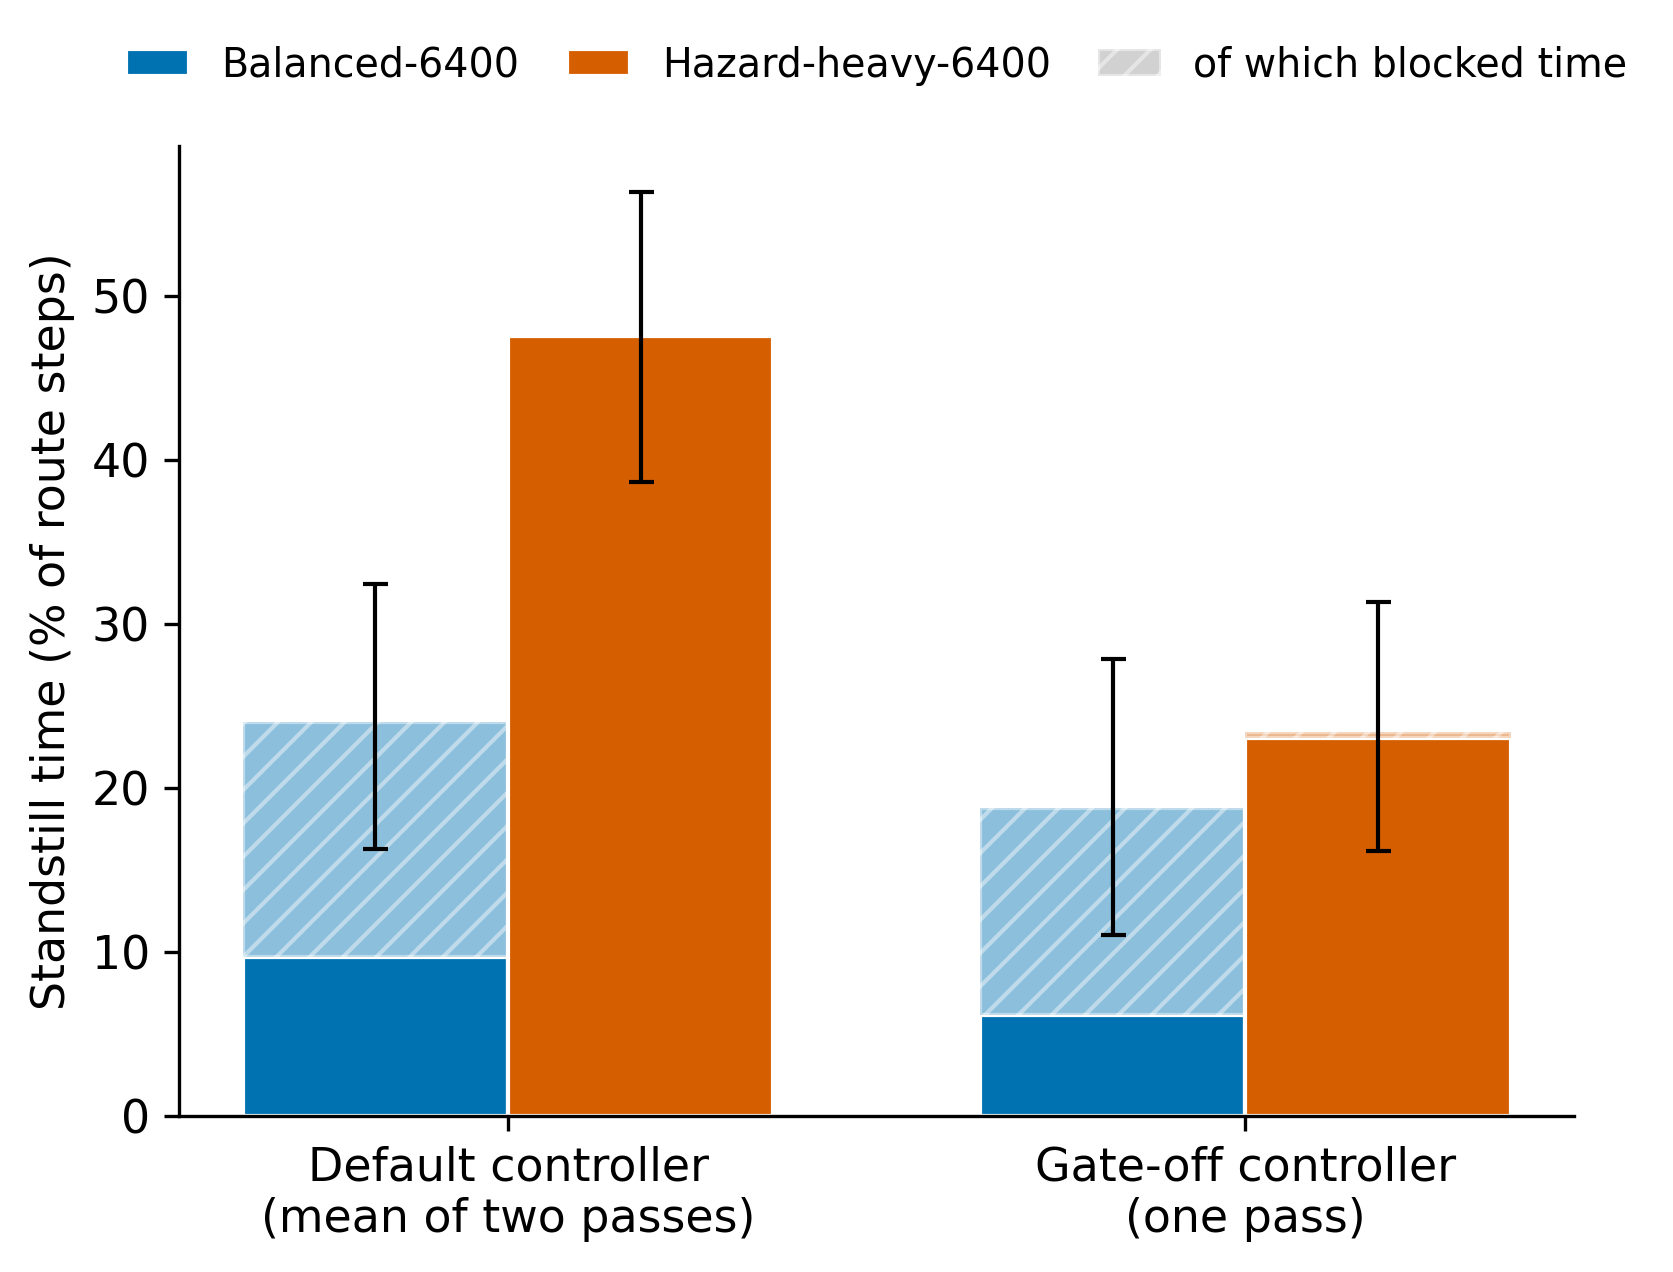
\includegraphics[width=\linewidth,height=0.8\textheight,keepaspectratio]{figure_5.png}
\caption{Mean standstill time of Golden-6400 and Flooded-6400 on the 44 routes under the default controller (mean of the two passes) and the gate-off controller (one pass). The hatched part of each bar is blocked time (at least 5 s commanded to accelerate without moving); the solid part is all other standstill. Error bars are 95 \% percentile bootstrap intervals over routes for the whole bar.}
\end{figure}

Is the rate of near-stationary plans a property of the model alone? No. Without the gate \texttt{Flooded\mbox{-}6400} returned such plans about half as often as with it (14.58 \% against 28.04 \%; \ensuremath{-}13.46 pp, CI [\ensuremath{-}19.34, \ensuremath{-}8.65]), with the same weights. The plans depend on the state, and the gate holds the vehicle at rest, where short plans are most frequent (Table 3). We read this as a feedback between gate and plans, which this run does not test directly: the gate turns a short plan into a held stop, and the held stop keeps the model in the states that return short plans. The rate on identical inputs (Section 4.2) does not depend on the controller.

What did removing the gate do to the outcomes? For \texttt{Flooded\mbox{-}6400} it exchanged waiting for progress and collisions at an unchanged score. Its route completion rose from 64.40 \% to 75.35 \% (+10.95 pp, CI [3.97, 18.02]), and it completed 24 routes against 16 and 18 in its two default passes. Its collision events per route rose from 0.49 to 0.91 (+0.42, CI [0.14, 0.72]), and its Driving Score did not change detectably (45.69 against 47.55; \ensuremath{-}1.87 points, CI [\ensuremath{-}10.16, 5.41]). For \texttt{Golden\mbox{-}6400} no outcome changed detectably (Driving Score 51.45 against 51.52; route completion 72.36 \% against 71.24 \%; 0.73 collision events per route in both). Between the checkpoints, without the gate, neither the Driving Score (+5.77 points, CI [\ensuremath{-}1.68, 13.84]) nor the route completion (\ensuremath{-}2.99 pp, CI [\ensuremath{-}9.92, 4.16]) nor the collision events per route (\ensuremath{-}0.18, CI [\ensuremath{-}0.45, 0.05]) differed detectably. Removing the gate is therefore not a remedy for the standstill of this checkpoint. The 60 s rule ended 4 routes of \texttt{Flooded\mbox{-}6400} without the gate against 10 and 7 in its two passes with it, and 6 routes of \texttt{Golden\mbox{-}6400} against 5 and 7. The added collision events of \texttt{Flooded\mbox{-}6400} were mainly with the road layout (+0.20 per route, CI [0.06, 0.36]). The distance within a common tick window, which the rule also lists, was not computed.

\subsection{The Decoupling Checkpoint}

Does the scenario mix or the manoeuvre mix carry the difference? \texttt{Decoupling\mbox{-}6400} has the scenario-group mix of the obstacle-heavy set and the manoeuvre mix and stationary share of the balanced set (Section 3.3). It was evaluated once on the 44 routes; all routes were scored at the first launch. Its readings were fixed before the checkpoint had run any route (ANALYSIS\_ADDENDUM \S{}6 and \S{}15) and are applied unchanged, with the per-route mean of the two passes of each of the other two checkpoints as comparator. The plan-level reading compares its share of near-stationary plans with that of each of the other two checkpoints. The mix may be called a candidate remedy only if it has fewer such plans than the obstacle-heavy checkpoint, no more blocked time and no lower Driving Score, each judged by its interval.

Its rate of near-stationary plans was not detectably different from that of the balanced checkpoint (Figure 3 shows the pooled distributions). \texttt{Decoupling\mbox{-}6400} returned a near-stationary plan in 1.58 \% of steps, against 28.04 \% for \texttt{Flooded\mbox{-}6400} (\ensuremath{-}26.47 pp, CI [\ensuremath{-}32.42, \ensuremath{-}20.84]) and 1.22 \% for \texttt{Golden\mbox{-}6400} (+0.36 pp, CI [\ensuremath{-}0.33, 1.74]), which closes 98.7 \% of the gap between the two. On the 37 routes without training overlap the two contrasts were \ensuremath{-}26.83 pp (CI [\ensuremath{-}33.26, \ensuremath{-}20.82]) and \ensuremath{-}0.13 pp (CI [\ensuremath{-}0.79, 0.56]), and against each pass of \texttt{Flooded\mbox{-}6400} alone the first was \ensuremath{-}25.23 and \ensuremath{-}27.71 pp. Among steps at 0.5 m/s or less the stay-put share was 0.68 \% against 26.03 \% for \texttt{Flooded\mbox{-}6400} (\ensuremath{-}25.35 pp, CI [\ensuremath{-}29.45, \ensuremath{-}21.62]; 39 routes). By the rule, near-stationary planning went with the manoeuvre mix and the stationary share, not with the scenario-group mix. Standstill time gave the same reading: 27.79 \% against 47.55 \% for \texttt{Flooded\mbox{-}6400} (\ensuremath{-}19.76 pp, CI [\ensuremath{-}28.97, \ensuremath{-}10.71]) and 24.01 \% for \texttt{Golden\mbox{-}6400} (+3.78 pp, CI [\ensuremath{-}3.86, 12.53]).

How far does this reading go? Three limits apply. First, the decoupling set shares 86.3 \% of its samples with the balanced set (5,523 of 6,400), and seed, schedule and pool are the same, so \texttt{Decoupling\mbox{-}6400} is not an independent repetition of \texttt{Golden\mbox{-}6400}. What it shows is that replacing the other 877 samples, so as to reach the scenario-group mix of the obstacle-heavy set, did not bring the near-stationary plans back. The set has the scenario-group shares of the obstacle-heavy set, but its observed brake and hazard shares (35.1 \% and 24.2 \%) are those of the balanced set (35.4 \% and 23.8 \%) and not those of the obstacle-heavy set (41.3 \% and 30.8 \%; Table 1). What was varied is therefore the scenario group from which the samples come, not how often they contain braking or a hazard. Second, the design fills three of four cells: no checkpoint has the balanced scenario-group mix with the manoeuvre mix and stationary share of the obstacle-heavy set. The statement that the difference does not go with the scenario-group mix therefore holds at the balanced manoeuvre mix and stationary share only. Third, among the low-speed samples of the decoupling set 11.1 \% stay put, as in the balanced set (10.9 \%) and unlike the obstacle-heavy set (30.9 \%). This agrees in direction with the conjecture of Section 3.2, although both checkpoints planned to stay put far less often than that share.

Is the decoupling mix a remedy? Not by the rule fixed in advance. Against \texttt{Flooded\mbox{-}6400} it had more blocked time (15.39 \% against 0.00 \%; +15.39 pp, CI [8.78, 24.42]; 15 routes), so the rule reads that the checkpoint trained on this mix had fewer near-stationary plans at a cost (one training run). Its route completion was higher (+7.06 pp, CI [2.37, 11.80]), its Driving Score was not (47.69 against 47.55; +0.14 points, CI [\ensuremath{-}5.90, 6.50]), and it had more collision events per route (+0.35, CI [0.06, 0.69]; 37 events in its one pass). Its Success Rate was 6.8 \% (3 of 44 routes). Against \texttt{Golden\mbox{-}6400} no measure differed detectably (blocked time +1.09 pp, CI [\ensuremath{-}5.95, 8.49]; Driving Score \ensuremath{-}3.83 points, CI [\ensuremath{-}11.06, 2.68]). The checkpoint has one training seed and one pass, and the two factors it shares with the balanced mix remain bundled.

\subsection{The 1,600-Sample Pair}

Does the difference between the mixes appear at 1,600 samples? In the plans it does, by a small margin. \texttt{Golden\mbox{-}1600} and \texttt{Flooded\mbox{-}1600} were run once on the 44 routes with the default controller; all routes were scored at the first launch. Three tests for this pair were fixed after \texttt{Golden\mbox{-}1600} had finished and while \texttt{Flooded\mbox{-}1600} was running, before any value of either run was computed (ANALYSIS\_ADDENDUM \S{}31, where they are named S1 to S3). N1, the primary test, is the share of steps with a near-stationary plan, with the rule of F1. N2 is the standstill time, read by the cases of F2. N3 is the Bench2Drive Driving Efficiency, met if the difference is positive, its interval lies above zero and p \ensuremath{<} 0.05; N2 and N3 are Holm-adjusted over the two. N1 was met: 4.92 \% for \texttt{Golden\mbox{-}1600} against 8.34 \% for \texttt{Flooded\mbox{-}1600} (\ensuremath{-}3.42 pp, CI [\ensuremath{-}7.74, \ensuremath{-}0.11], p = 0.047). The interval ends close to zero and the p-value lies close to its threshold, so we report a difference that is present and small. It has the direction and about the size of the difference on identical replayed inputs (\ensuremath{-}2.75 pp, Section 4.2); that replay value was known when the tests were fixed. The test is exact, and no route had a zero difference.

Does it reach the motion of the vehicle? The evidence is as close to the border as for the plans. Standstill time was 24.93 \% against 33.41 \% (\ensuremath{-}8.49 pp, CI [\ensuremath{-}17.19, 0.46], Holm p = 0.030): the rank test rejects and the interval of the mean includes zero, which the rule of N2 reads as inconclusive. N1 passes its rule by a narrow margin and N2 fails its rule by a narrow margin, so the two verdicts are not a contrast between plans and motion; in one pass, both differences are small and at the border of detection. The Bench2Drive Driving Efficiency did not differ detectably (97.83 against 102.30; \ensuremath{-}4.47 points, CI [\ensuremath{-}16.61, 2.29], p = 0.19; 43 routes; N3 is not met), and its sign is opposite to that of the 6,400-sample pair. Blocked time was low in both checkpoints (1.26 \% and 1.90 \%). Driving Score (52.83 against 46.56; +6.27 points, CI [\ensuremath{-}3.21, 17.69]), route completion (69.92 \% against 74.33 \%; \ensuremath{-}4.40 pp, CI [\ensuremath{-}12.46, 3.14]) and collision events (29 against 38; \ensuremath{-}0.20 per route, CI [\ensuremath{-}0.55, 0.14]) did not differ detectably; the infraction penalty factor was higher for \texttt{Golden\mbox{-}1600} (0.74 against 0.61; +0.13, CI [0.04, 0.24]). Each checkpoint completed 20 routes, and the Success Rate was 18.2 \% and 15.9 \%.

Is the difference smaller than at 6,400 samples? Yes, on all three tested measures. The difference of the 6,400-sample pair (mean of its two passes) minus that of the 1,600-sample pair was \ensuremath{-}23.41 pp for near-stationary plans (CI [\ensuremath{-}31.39, \ensuremath{-}15.49]), \ensuremath{-}15.05 pp for standstill time (CI [\ensuremath{-}26.97, \ensuremath{-}4.16]) and +26.99 points for Driving Efficiency (CI [10.56, 40.03]; 41 routes). The low-speed stay-put shares of the two 1,600-sample sets differ almost as much as those of the 6,400-sample sets (Table 1), so the training share alone does not account for the size of the difference. The 1,600-sample checkpoints had a quarter of the optimizer steps (Section 3.4), and the design cannot separate the number of samples from the number of steps.

Where do the two checkpoints lie relative to the unadapted policy (descriptive)? \texttt{Golden\mbox{-}1600} returned fewer near-stationary plans than \texttt{Base\mbox{-}Rerun} (13.24 \%), by \ensuremath{-}8.32 pp (CI [\ensuremath{-}13.98, \ensuremath{-}3.90]); for \texttt{Flooded\mbox{-}1600} the difference was not detectable (\ensuremath{-}4.90 pp, CI [\ensuremath{-}11.43, 1.02]). The rise above the unadapted policy that \texttt{Flooded\mbox{-}6400} shows in closed loop (Section 4.7) is therefore not seen in closed loop at 1,600 samples. The Driving Score of \texttt{Golden\mbox{-}1600} was 52.83 against 42.60 for \texttt{Base\mbox{-}Rerun} (+10.23 points, CI [1.06, 21.69]; Wilcoxon p = 0.19). The interval and the test disagree, and the comparison is one pass without a rule fixed in advance, so we do not read it as an established gain. Each 1,600-sample checkpoint has one training seed and one pass, and its training run was interrupted and resumed, so no pass-to-pass variation is available for this pair.

\subsection{The Fine-Tuned Checkpoints against the Unadapted Policy (Post Hoc)}

Did fine-tuning move the policy toward staying put or away from it? In both directions in these checkpoints: the one trained on the balanced mix lay below the unadapted policy and the one trained on the obstacle-heavy mix above it. This comparison was added after the first pass was known and has no decision rule. The unadapted policy has one pass under the current termination rule (\texttt{Base\mbox{-}Rerun}, Section 4.1), so its own pass-to-pass variation is not averaged out. \texttt{Base\mbox{-}Rerun} returned a near-stationary plan in 13.24 \% of steps (mean of per-route shares; Figure 3 shows the pooled distribution). \texttt{Golden\mbox{-}6400} lay below it (1.22 \% over both passes; \ensuremath{-}12.02 pp, CI [\ensuremath{-}18.04, \ensuremath{-}7.75]) and \texttt{Flooded\mbox{-}6400} above it (28.04 \%; +14.80 pp, CI [7.95, 21.62]), as on identical inputs (Section 4.2). Standstill time followed: \ensuremath{-}12.27 pp for \texttt{Golden\mbox{-}6400} (CI [\ensuremath{-}21.55, \ensuremath{-}3.85]) and +11.27 pp for \texttt{Flooded\mbox{-}6400} (CI [1.00, 20.86]), against 36.28 \% for \texttt{Base\mbox{-}Rerun}.

Did fine-tuning raise the benchmark score? For \texttt{Golden\mbox{-}6400} the evidence is indicative. Its Driving Score over both passes was 51.52 against 42.60 (+8.92 points, CI [0.96, 18.04], p = 0.058): the interval excludes zero and the Wilcoxon test does not reject. In the first pass alone the difference was +11.42 (CI [2.83, 21.62]) and in the second +6.41 (CI [\ensuremath{-}2.07, 15.89]). Its route completion did not differ from that of \texttt{Base\mbox{-}Rerun} (\ensuremath{-}0.68 pp, CI [\ensuremath{-}10.02, 8.51]); the difference in score came with fewer collision events per route (0.73 against 1.11; \ensuremath{-}0.39, CI [\ensuremath{-}0.78, \ensuremath{-}0.09]) and with more blocked time (+13.93 pp, CI [7.37, 23.77]). For \texttt{Flooded\mbox{-}6400} the Driving Score difference had an interval that includes zero (+4.95, CI [\ensuremath{-}5.26, 14.44]), with fewer collision events per route (\ensuremath{-}0.62, CI [\ensuremath{-}1.00, \ensuremath{-}0.31]) and a route completion that was not detectably lower (\ensuremath{-}7.52 pp, CI [\ensuremath{-}17.59, 2.32]). \texttt{Decoupling\mbox{-}6400}, with one pass, had a Driving Score difference of +5.09 (CI [\ensuremath{-}4.73, 15.00]).

\subsection{Motion-History Swap Test (Exploratory)}

Protocol. The usual account of the inertia problem is that a stay-put plan follows the policy's own recent motion and not the scene \cite{ref12}. The only non-visual motion input of the model is the ego history of Section 3.1. This exploratory test replaced that input on about one step in five, on a schedule fixed in advance and identical for every route and checkpoint, and read the plan that the model returned. On a step at 0.5 m/s or less the history was replaced by a *moving history*, a straight line behind the vehicle at a constant 4.0 m/s; on a step above 0.5 m/s it was replaced by a *stationary history* with all positions at zero. The camera frames and the navigation command were sent unchanged. The plan of a replaced step was logged and not acted on: the vehicle received the command of the previous step. \texttt{Flooded\mbox{-}6400} and \texttt{Golden\mbox{-}6400} were each run once on eight routes with this agent; all 16 routes were scored at the first launch. The outcomes, their reading and the limits below were fixed before any run with a replaced history existed and were not changed afterwards (ANALYSIS\_ADDENDUM \S{}11, \S{}11-B and \S{}32); a preliminary evaluation with this test preceded the runs of this section.

Outcomes. Because the waypoints are integrated from an initial speed $v_0$ that is itself estimated from the ego history (Section 3.1), a replaced history changes the extent $L$ mechanically, whatever the learned controls are. The outcomes are therefore defined on the planned change of speed, which depends on the learned accelerations and not on $v_0$: $\Delta v = v_{\text{end}} - v_{\text{start}}$, where $v_{\text{start}}$ is the distance to the first waypoint divided by 0.1 s and $v_{\text{end}}$ the path length between waypoints 54 and 64 divided by 1.0 s. A plan *holds speed* if $|\Delta v| < 0.5$ m/s, *accelerates* if $\Delta v \ge 0.5$ m/s and *decelerates* if $\Delta v \le -0.5$ m/s; it *ends at rest* if $v_{\text{end}} < 0.5$ m/s. Among steps at 0.5 m/s or less, W-a (primary) is the share of plans that hold speed under the moving history minus that share under the true history, and W-b is the same difference for plans that end at rest. Shares are per route, a route counts with at least 20 steps in both conditions, and a checkpoint with fewer than five such routes receives no reading. By the rule, the learned controls *depend on the ego history* if the interval of W-a excludes zero. The rule allows the stay-put plans to be tied to a history that reports rest only if, in addition, the share of plans that hold speed is lower under the moving history.

Do the controls of the obstacle-heavy checkpoint depend on the ego history? They do, and not in the direction that this rule names. On the six routes that count, \texttt{Flooded\mbox{-}6400} planned to hold its speed in 84.29 \% of the steps with the moving history and in 52.29 \% of the steps with the true history (W-a: +32.00 pp, CI [22.63, 36.04], Wilcoxon p = 0.031, the smallest value possible with six routes). It planned to accelerate in 15.71 \% against 47.65 \% (\ensuremath{-}31.93 pp, CI [\ensuremath{-}36.12, \ensuremath{-}22.59]). The interval of W-a excludes zero, so the learned controls depend on the ego history. The share of plans that hold speed rose under the moving history and did not fall, so the condition for tying the stay-put plans to a history that reports rest is not met, and we report the outcome as found: told that it was moving at 4.0 m/s, this checkpoint more often planned to keep that speed and less often planned to accelerate. Leaving out the true-history steps that directly follow a replaced step gave the same reading (+32.37 pp, CI [22.28, 36.54]).

Are the stay-put plans matched by braking plans? They are not. With the true history, 44.76 \% of the plans of \texttt{Flooded\mbox{-}6400} at low speed ended at rest; with the moving history none did (W-b: \ensuremath{-}44.76 pp, CI [\ensuremath{-}50.51, \ensuremath{-}36.42], p = 0.031), and none decelerated. In the situations in which this checkpoint planned to stay where it was, it did not plan to brake when its history reported motion. In this action space a plan that stays put at rest is a plan without acceleration, so this outcome is expected if the controls do not change, and by the rule it is not by itself evidence that the model uses the history.

What about the balanced checkpoint? There is no reading. \texttt{Golden\mbox{-}6400} was rarely at low speed, and only three of its eight routes had 20 steps in both conditions. Pooled over its low-speed steps it planned to accelerate in 97.95 \% of 1,168 steps with the moving history and in 96.71 \% of 4,405 steps with the true history, and to hold speed in 2.05 \% against 2.95 \%.

What happened with a stationary history on steps where the vehicle was moving (descriptive, eight routes)? From a stationary history the integration starts at $v_0 = 0$, so a plan that ends at rest is here a plan without acceleration from rest, not a braking plan. \texttt{Flooded\mbox{-}6400} returned such a plan in 30.22 \% of these steps against 0.08 \% with the true history (+30.14 pp, CI [16.58, 42.00]), and \texttt{Golden\mbox{-}6400} in 3.05 \% against 0.00 \% (+3.05 pp, CI [0.30, 8.11]). The two checkpoints were not compared by a test on these steps, and these values carry no reading.

Limits. The test replaced the ego-history tokens only. The camera window, which also shows whether the vehicle moves, was unchanged, so a visual route to the same behaviour was not tested. A moving history with camera frames that show no motion is an input the model was not trained on, and so is the reverse. A replaced step measures the immediate plan, not how long a stop lasts. Holding the previous command on one step in five alters the closed loop, so the scores and the standstill time of these runs are not comparable with any other run and are not analysed. The test has eight routes, one pass and unseeded sampling, and with six usable routes its Wilcoxon test cannot give a value below 0.031. Three readings of W-a are not separated. A policy that uses its speed correctly would also plan to accelerate less often when its history reports 4.0 m/s. The class of plans that hold speed covers staying at rest under the true history and keeping 4.0 m/s under the moving one, which are different behaviours. And the outcome may be the response of the model to an input it has not seen. No reference model was run with this agent: \texttt{Golden\mbox{-}6400} gave no reading and the unadapted policy was not tested.

\section{Discussion and Limitations}

The two 6,400-sample checkpoints differed by \ensuremath{-}26.83 pp over both passes in how often they returned a near-stationary plan. The difference recurred in a second pass. A difference in stay-put plans ($L < 0.64$ m) in the same direction was present on identical replayed inputs (Section 4.2) and among steps at rest (Table 3). A second pass addresses evaluation noise, not variation between training runs, and with one checkpoint per mix we cannot separate the effect of the mix from that of the training run. Two observations bear on this, and neither removes it. First, \texttt{Decoupling\mbox{-}6400}, trained in a separate run, returned near-stationary plans about as rarely as the balanced checkpoint (1.58 \% against 1.22 \% of steps), so that in the three design cells that were run the rate went with the manoeuvre mix and the stationary share, not with the scenario-group shares. Its set shares 86.3 \% of its samples with the balanced set, so this is closer to a second run on nearly the same data than to an independent test. Second, on identical inputs the unadapted policy lay between the two fine-tuned checkpoints, and the closed-loop runs gave the same order (Section 4.7). This gives the direction of each checkpoint relative to its starting point; it does not bear on variation between training runs. Of the five fine-tuned checkpoints only \texttt{Flooded\mbox{-}6400} lay detectably above the unadapted policy in closed loop. Each mix still has one seed, and the two remaining factors are bundled. At 1,600 samples the difference was far smaller and at the border of detection (Section 4.6).

The behaviour matches the description of the inertia problem by Codevilla et al. \cite{ref12}: a policy that, once slow, keeps predicting that it stays where it is. The match is behavioural. We do not show that the stops of \texttt{Flooded\mbox{-}6400} were unwarranted, and on the replayed states \texttt{Golden\mbox{-}6400} stayed put less often than the demonstrations themselves (0.63 \% of plans against 3.91 \% of demonstrated futures, pooled over the states), so the comparison ranks the checkpoints by how often they stay put and not by how well they drive. The behaviour is consistent with the conjecture of Section 3.2 that a flow-matching expert samples stay-put futures in low-speed contexts at a rate that rises with their share in the training data. The conjecture, however, does not account for \texttt{Golden\mbox{-}6400} planning to stay put far less often than its own training share, nor for the small size of the difference at 1,600 samples, where the training shares differ almost as much as at 6,400 (Section 4.6), and it holds only in the limit of exact sampling, from which the four-evaluation sampler is far; a pull of coarse sampling toward the conditional mean is a rival mechanism that we did not test. The conjecture of Section 3.2 is a data-side reading of the inertia problem for a sampling head, not a rival to it. In this action space a plan that stays put at rest is a plan without acceleration (Section 3.1), so the difference can also be read as a difference in how often the model issues a start.

Section 4.8 reports an exploratory test in which the ego-motion history of the model was replaced. Its outcome is reported as found. With a history that reported motion at 4.0 m/s, \texttt{Flooded\mbox{-}6400} planned to hold its speed more often (+32.00 pp, CI [22.63, 36.04]; six routes) and to accelerate less often, so by the rule fixed in advance its learned controls depend on the ego history. This does not identify why the checkpoint stays put. The rule's condition for tying the stay-put plans to a history that reports rest was not met. A policy that uses its speed correctly would also accelerate less when it is told that it already moves, the class of plans that hold speed covers two different behaviours, and the replaced input is one the model was not trained on (Section 4.8). No reference model was tested: \texttt{Golden\mbox{-}6400} gave no reading and the unadapted policy was not run. The test replaced only the ego-history tokens; the camera window, which also shows that the vehicle is at rest, was unchanged, so a visual route to the same behaviour was not tested.

The controller decides how much of the difference in plans becomes a difference in standstill. The gate turns a short plan into a held stop. With the gate removed, the difference between the two checkpoints in time below 0.1 m/s shrank to \ensuremath{-}4.65 pp (CI [\ensuremath{-}11.44, 3.20]; the rank test still rejects, p = 0.0048), against \ensuremath{-}23.54 pp with the gate, while the difference in near-stationary plans (\ensuremath{-}13.99 pp, CI [\ensuremath{-}20.27, \ensuremath{-}9.52]) and in time below 1.0 m/s (\ensuremath{-}21.40 pp, CI [\ensuremath{-}28.67, \ensuremath{-}12.77]) remained (Section 4.4). This supports an origin of the difference in the plans, with the gate amplifying its expression as full stops (exploratory, one pass). The gate may also feed back on the plans: without it the obstacle-heavy checkpoint returned near-stationary plans about half as often, with the same weights, so the closed-loop rate of such plans describes the model together with its controller. Total standstill also adds two things that moved in opposite directions. Under both controllers the balanced checkpoint had less standstill in which the controller was not asking for acceleration, and more time in which it was commanded to accelerate and did not move. Removing the gate was not a remedy for the obstacle-heavy checkpoint: it completed more of each route (+10.95 pp, CI [3.97, 18.02]) with more collision events per route (+0.42, CI [0.14, 0.72]) and no detectable change in Driving Score. Que et al. \cite{ref48} report the same pattern for a release rule on a different planner. Neither a held stop nor a blocked vehicle solves those scenarios.

Less standstill showed as higher driving efficiency (post hoc), not as a higher Driving Score. Over both passes the balanced checkpoint completed more of each route (+6.84 pp, CI [0.80, 13.29]), and its Driving Score was not detectably higher (+3.96 points, CI [\ensuremath{-}3.06, 11.67]). It was more efficient: its Bench2Drive Driving Efficiency was higher by 22.89 points (CI [6.14, 34.89]), and on the routes that both checkpoints completed it needed 45.62 s against 76.51 s (Section 4.3). These two comparisons are post hoc and descriptive: they were added after the Driving Score had shown no detectable difference. The Driving Efficiency leaves out a final stop and does not count blocked time as a cost (Section 4.3), and at 1,600 samples the pre-specified test on it was not met, with a point estimate of the opposite sign (Section 4.6). The first pass alone had shown a gain of +10.52 points, which did not recur (second pass \ensuremath{-}2.59, CI [\ensuremath{-}11.94, 6.51]). One pass of 44 routes is therefore not enough to compare two checkpoints on Driving Score: the obstacle-heavy checkpoint itself differed by 8.09 points between its two passes (CI [1.93, 15.16]). Collision events per route did not differ detectably over both passes (+0.24, CI [0.00, 0.43]; 28 against 28 events in the first pass and 36 against 15 in the second), and per distance driven the difference was not detectable (ratio 1.29, CI [0.90, 1.92]). \texttt{Decoupling\mbox{-}6400} showed the same pattern against the obstacle-heavy checkpoint: far fewer near-stationary plans, more blocked time, more route completion and no detectable difference in Driving Score (Section 4.5). We therefore describe the balanced 6,400-sample checkpoint as more efficient by this post hoc measure, at a Driving Score and a collision count that were not detectably different, not as driving better, and with three checkpoints we do not describe a trade-off curve. The results are consistent with a trade-off between standing still and progress, in which the checkpoint that stands still less advances farther and spends more time commanded to move without moving, at places where a collision was recorded. Whether a stop was required in a given situation is not known from our logs, so less standstill cannot be read as better, and we do not recommend one mix over the other. For evaluation practice three points follow. The standstill fraction should be reported split by command and next to collisions, because on its own it counts a vehicle that is commanded to move and does not the same as one that is holding; this needs only the speed, the throttle, the brake and the planned trajectory of each step in the log. A several-fold difference in plans did not show in the Driving Score. And comparisons on that score need repeated passes, as stated above.

Limitations.

Design. Each condition is one checkpoint from one training run (seed 42), and the 1,600-sample runs were interrupted and resumed. All intervals describe route-to-route variation for these checkpoints, not variation between training runs, so the effect of a mix cannot be separated from that of its training run. The mixes differ in group mix, lateral balance and stationary share together. The decoupling checkpoint separates only the scenario-group mix, and it has one seed and one evaluation pass. We studied one policy, one simulator and one controller.

Evaluation. Closed-loop runs are not deterministic. The per-route standstill differed between the two passes of the same checkpoint with a standard deviation of 18 to 25 pp (Section 4.1). One server process served all routes of a job without clearing its streaming cache, and two processes of the same model did not return identical plans on all replayed states, for a reason we did not find (Section 4.2). A difference between two jobs therefore includes a difference between two server processes. The second pass and the same-input replay address this for the 6,400-sample pair; the results with one pass (the decoupling checkpoint, the runs without the gate, the 1,600-sample pair and the unadapted policy) remain exposed to it. Their contrasts in Driving Score and in collision events also carry the pass-to-pass variation shown in Section 4.3, where a first-pass gain in Driving Score did not recur, and are descriptive. The 44 routes are a subset of the benchmark, seven of them are touched by training samples, and the controller was tuned on 20 of them with a fine-tuned checkpoint, which can favour fine-tuned models over the unadapted one. The gate-off controller was written after first results of these checkpoints were known. The 60 s standstill rule censors the standstill fraction (Section 4.1). With this subset, our controller, Low rendering quality and CARLA 0.9.15, the Driving Scores and the Driving Efficiency are not comparable with published 220-route results.

Measurement and transfer. Blocked time is inferred from the command log, not from a contact sensor, and the bridge logs neither signal state nor actor distances, so we cannot say whether a stop was required. Scripted CARLA traffic does not react to an ego vehicle that waits or is blocked the way human drivers would, so the costs that either behaviour imposes on others are not represented. Inference uses a VLM quantized to 4-bit weights and 8-bit activations and streaming key-value cache reuse, whereas training uses full-context BF16. The training data were collected at rendering quality Epic and evaluation ran at Low; the collection quality is taken from the collection code, and we have no log of the collection run itself. The evaluated models therefore saw images of lower quality than their training images, a visual domain shift that may affect all fine-tuned models and could moderate the differences we report. We did not compare against controller-side anti-stall rules or model-side remedies such as history dropout \cite{ref27} or speed prediction \cite{ref12}.

Pre-specification. The tests were fixed after preliminary evaluations of the same checkpoints on the same routes (Section 4.1). They are pre-specified tests on new runs, not tests of hypotheses formed without sight of related data, and the route set was not held out.

Future work follows from these limits: further seeds for the 6,400-sample pair and for the decoupling model; per-context sampling of many noise seeds at logged low-speed states to measure the stay-put sampling rate directly; evaluation of the matched pair on the remaining routes; logging of contact and of hazards ahead, so that a stop can be classed as required or not; and a comparison with history dropout and with a creep-style controller.

\section{Conclusion, Availability and Disclosures}

We compared two fine-tuning mixes, drawn from the same verified pool, for the flow-matching action expert of Alpamayo 1.5, with one training run per mix and dataset size. The obstacle-heavy 6,400-sample checkpoint returned a near-stationary plan in 26.80 \% of steps and the balanced one in 1.31 \%. A test fixed before the runs was met (\ensuremath{-}25.49 pp, CI [\ensuremath{-}31.69, \ensuremath{-}19.63]), a repeat test on a second pass was met (\ensuremath{-}28.16 pp, CI [\ensuremath{-}34.81, \ensuremath{-}21.75]), and a difference in stay-put plans in the same direction was present on identical replayed inputs, where the unadapted policy lay between the two checkpoints, as it did in closed loop. This behaviour matches the description of the inertia problem; we do not show that the stops were unwarranted. A third checkpoint, with the scenario-group shares of the obstacle-heavy set and the manoeuvre mix and stationary share of the balanced set, returned near-stationary plans about as rarely as the balanced checkpoint (1.58 \% of steps; three of the four cells of this design were run), so in these three training runs the rate went with the manoeuvre mix and the stationary share. On the road the balanced checkpoint stood still about half as long, completed more of each route and drove at a higher speed relative to the surrounding traffic (Driving Efficiency +22.89 points, CI [6.14, 34.89]; post hoc, and the test of this measure at 1,600 samples was not met). It spent more time commanded to accelerate without moving and did not obtain a detectably higher Driving Score (+3.96 points over both passes, CI [\ensuremath{-}3.06, 11.67]); a gain seen in the first pass did not recur in the second, and collision events did not differ detectably per route (+0.24, CI [0.00, 0.43]) or per distance driven. Without the controller's standstill gate the difference in full stops shrank to \ensuremath{-}4.65 pp (CI [\ensuremath{-}11.44, 3.20]; the rank test still rejects, p = 0.0048) and the difference in near-stationary plans remained (\ensuremath{-}13.99 pp, CI [\ensuremath{-}20.27, \ensuremath{-}9.52]), which supports an origin of the difference in the plans, with the gate turning short plans into held stops (exploratory, one pass). By the rule fixed in advance the checkpoint trained on the decoupling mix had fewer near-stationary plans at a cost (one training run), and the mix is not called a remedy. At 1,600 samples the differences were smaller and at the border of detection: \ensuremath{-}3.42 pp in near-stationary plans (CI [\ensuremath{-}7.74, \ensuremath{-}0.11]) and \ensuremath{-}8.49 pp in standstill time (CI [\ensuremath{-}17.19, 0.46]). In an exploratory test on six routes the learned controls of the obstacle-heavy checkpoint depended on its ego-motion history (plans that hold speed: +32.00 pp under a history that reports motion, CI [22.63, 36.04]). The test does not identify the mechanism: the pre-specified condition for tying the stay-put plans to a history that reports rest was not met, correct use of speed would give the same outcome, and the camera input was not varied. For evaluation practice, standstill time should be reported split by command, and a comparison on Driving Score needs repeated passes. With one checkpoint per mix the dependence on composition across training seeds is untested. We make no safety claim.

\textbf{Data availability.} The four Matrix fine-tuning datasets and the decoupling dataset are on the Hugging Face Hub as \nolinkurl{earth37815/lead-alpamayo-pai_matrix_golden_1600}, \nolinkurl{earth37815/lead-alpamayo-pai_matrix_golden_6400}, \nolinkurl{earth37815/lead-alpamayo-pai_matrix_flooded_1600}, \nolinkurl{earth37815/lead-alpamayo-pai_matrix_flooded_6400} and \nolinkurl{earth37815/lead-alpamayo-pai_matrix_floodedgroups_balanced_6400}. Each dataset card states its composition, construction and evaluation-route overlap. Route-level records, step logs and trainer artifacts are archived at \pending{[[PENDING: archive DOI]]}.

\textbf{Code availability.} The analyses of this paper are produced by the scripts \texttt{scripts/evaluation/fullload\_*.py} and \nolinkurl{scripts/evaluation/same_input_replay.py}, which use the definitions and statistics of \nolinkurl{scripts/evaluation/paper_reanalysis.py} and write every reported number to result files in \nolinkurl{docs/provenance/}. The rules fixed before each analysis are in \nolinkurl{docs/ANALYSIS_ADDENDUM.md}. The full-loading server is \nolinkurl{scripts/evaluation/flashdrive_server_fullpatch.py}. All are in the project repository at commit \pending{[[PENDING: commit hash]]}. Fine-tuning follows the open-source Alpamayo recipe (\nolinkurl{NVlabs/alpamayo-recipes}, seed 42) \cite{ref20}.

\textbf{Author contributions.} \pending{[[PENDING: CRediT statement from the authors]]}

\textbf{Funding.} \pending{[[PENDING: funding statement from the authors]]}

\textbf{Competing interests.} \pending{[[PENDING: statement from the authors]]}

\textbf{Ethics.} The study used a driving simulator only. It involved no human participants, no animals and no personal data.

\textbf{AI assistance disclosure.} Generative AI tools were used throughout this work: to write and revise the analysis scripts, the evaluation queue scripts and the controller variants used in the ablations; to propose and word the decision rules of the analysis addendum; to search and check the literature and the reference list; to check reported numbers against the analysis output; and to draft and revise the text of this manuscript. Most commits of the revision were made with AI assistance. \pending{[[PENDING: authors' statement on their own verification and responsibility]]}

\begin{thebibliography}{49}
\bibitem{ref1} Physical Intelligence, K. Black, N. Brown, J. Darpinian, K. Dhabalia, D. Driess, et al., "\ensuremath{\pi}0.5: a Vision-Language-Action Model with Open-World Generalization," arXiv preprint arXiv:2504.16054, Apr. 2025.
\bibitem{ref2} NVIDIA, Y. Wang, W. Luo, J. Bai, Y. Cao, et al., "Alpamayo-R1: Bridging Reasoning and Action Prediction for Generalizable Autonomous Driving in the Long Tail," arXiv preprint arXiv:2511.00088, 2025.
\bibitem{ref3} X. Jia, Z. Yang, Q. Li, Z. Zhang, and J. Yan, "Bench2Drive: Towards multi-ability benchmarking of closed-loop end-to-end autonomous driving," in Advances in Neural Information Processing Systems (NeurIPS), vol. 37, 2024, pp. 819--844.
\bibitem{ref4} Y. Hu et al., "Planning-oriented Autonomous Driving," in Proceedings of the IEEE/CVF Conference on Computer Vision and Pattern Recognition (CVPR), Vancouver, BC, Canada, 2023, pp. 17853--17862.
\bibitem{ref5} B. Jiang et al., "VAD: Vectorized Scene Representation for Efficient Autonomous Driving," in Proceedings of the IEEE/CVF International Conference on Computer Vision (ICCV), 2023, pp. 8340--8350.
\bibitem{ref6} C. Sima et al., "DriveLM: Driving with Graph Visual Question Answering," in Computer Vision -- ECCV 2024, Cham, Switzerland: Springer, 2024, pp. 256--274, doi: 10.1007/978-3-031-72943-0\_15.
\bibitem{ref7} H. Shao, Y. Hu, L. Wang, G. Song, S. L. Waslander, Y. Liu, and H. Li, "LMDrive: Closed-Loop End-to-End Driving with Large Language Models," in Proceedings of the IEEE/CVF Conference on Computer Vision and Pattern Recognition (CVPR), 2024, pp. 15120--15130.
\bibitem{ref8} Y. Lipman, R. T. Q. Chen, H. Ben-Hamu, M. Nickel, and M. Le, "Flow Matching for Generative Modeling," in Proc. Int. Conf. Learn. Represent. (ICLR), 2023.
\bibitem{ref9} A. Dosovitskiy, G. Ros, F. Codevilla, A. Lopez, and V. Koltun, "CARLA: An open urban driving simulator," in Proc. 1st Annu. Conf. Robot Learning (CoRL), 2017, pp. 1--16.
\bibitem{ref10} L. Nguyen, M. Fauth, B. Jaeger, D. Dauner, M. Igl, A. Geiger, and K. Chitta, "LEAD: Minimizing Learner--Expert Asymmetry in End-to-End Driving," in Proceedings of the IEEE/CVF Conference on Computer Vision and Pattern Recognition (CVPR), 2026, pp. 39775--39785, arXiv:2512.20563.
\bibitem{ref11} H. Caesar, V. Bankiti, A. H. Lang, S. Vora, V. E. Liong, Q. Xu, A. Krishnan, Y. Pan, G. Baldan, and O. Beijbom, "nuScenes: A multimodal dataset for autonomous driving," in Proceedings of the IEEE/CVF Conference on Computer Vision and Pattern Recognition (CVPR), 2020, pp. 11621--11631.
\bibitem{ref12} F. Codevilla, E. Santana, A. M. López, and A. Gaidon, "Exploring the Limitations of Behavior Cloning for Autonomous Driving," in Proceedings of the IEEE/CVF International Conference on Computer Vision (ICCV), 2019, pp. 9329--9338.
\bibitem{ref13} P. de Haan, D. Jayaraman, and S. Levine, "Causal Confusion in Imitation Learning," in Advances in Neural Information Processing Systems (NeurIPS), vol. 32, 2019, pp. 11698--11709.
\bibitem{ref14} Y. Liang, H. Chen, Z. Zhang, S. Han, and Z. Liu, "ParoQuant: Pairwise Rotation Quantization for Efficient Reasoning LLM Inference," in Proc. Int. Conf. Learn. Represent. (ICLR), 2026, arXiv:2511.10645.
\bibitem{ref15} Z. Li, Y. Liang, H. Zhang, J. Chen, Y. Liang, and Z. Liu, "FlashDrive: Flash Vision-Language-Action Inference for Autonomous Driving," arXiv preprint arXiv:2608.12932, 2026.
\bibitem{ref16} S. Ross, G. J. Gordon, and J. A. Bagnell, "A Reduction of Imitation Learning and Structured Prediction to No-Regret Online Learning," in Proceedings of the Fourteenth International Conference on Artificial Intelligence and Statistics (AISTATS), PMLR, vol. 15, 2011, pp. 627--635.
\bibitem{ref17} J.-T. Zhai, Z. Feng, J. Du, Y. Mao, J.-J. Liu, Z. Tan, Y. Zhang, X. Ye, and J. Wang, "Rethinking the Open-Loop Evaluation of End-to-End Autonomous Driving in nuScenes," arXiv preprint arXiv:2305.10430, 2023.
\bibitem{ref18} Z. Li, Z. Yu, S. Lan, J. Li, J. Kautz, T. Lu, and J. M. Álvarez, "Is Ego Status All You Need for Open-Loop End-to-End Autonomous Driving?" in Proceedings of the IEEE/CVF Conference on Computer Vision and Pattern Recognition (CVPR), 2024, pp. 14864--14873.
\bibitem{ref19} NVIDIA Research (NVlabs), "Alpamayo 1.5 (Alpamayo-1.5-10B): Open-Source Vision-Language-Action Driving Model and Codebase," GitHub and HuggingFace Repository (\nolinkurl{NVlabs/alpamayo1.5}, \nolinkurl{nvidia/Alpamayo-1.5-10B}), Mar. 2026.
\bibitem{ref20} NVIDIA Research (NVlabs), "Alpamayo Recipes: Supervised Fine-Tuning (SFT) and Reinforcement-Learning Post-Training Recipes for Alpamayo Models," GitHub repository (\nolinkurl{NVlabs/alpamayo-recipes}, recipe \texttt{alpamayo1\_5\_sft}, configuration \texttt{sft\_stage2\_nav}), 2026.
\bibitem{ref21} A. Prakash, K. Chitta, and A. Geiger, "Multi-Modal Fusion Transformer for End-to-End Autonomous Driving," in Proceedings of the IEEE/CVF Conference on Computer Vision and Pattern Recognition (CVPR), 2021, pp. 7077--7087.
\bibitem{ref22} Z. Zhang, A. Liniger, D. Dai, F. Yu, and L. Van Gool, "End-to-End Urban Driving by Imitating a Reinforcement Learning Coach," in Proceedings of the IEEE/CVF International Conference on Computer Vision (ICCV), 2021, pp. 15222--15232, arXiv:2108.08265.
\bibitem{ref23} Z. Li, K. Li, et al., "Hydra-MDP: End-to-end Multimodal Planning with Multi-target Hydra-Distillation," arXiv preprint arXiv:2406.06978, 2024.
\bibitem{ref24} K. Renz, L. Chen, E. Arani, and O. Sinavski, "SimLingo: Vision-Only Closed-Loop Autonomous Driving with Language-Action Alignment," in Proceedings of the IEEE/CVF Conference on Computer Vision and Pattern Recognition (CVPR), 2025, pp. 11993--12003, arXiv:2503.09594.
\bibitem{ref25} C. Wen, J. Lin, T. Darrell, D. Jayaraman, and Y. Gao, "Fighting Copycat Agents in Behavioral Cloning from Observation Histories," in Advances in Neural Information Processing Systems (NeurIPS), vol. 33, 2020, pp. 2564--2575.
\bibitem{ref26} K. Black et al. (Physical Intelligence), "\ensuremath{\pi}0: A Vision-Language-Action Flow Model for General Robot Control," arXiv preprint arXiv:2410.24164, 2024.
\bibitem{ref27} M. Bansal, A. Krizhevsky, and A. Ogale, "ChauffeurNet: Learning to Drive by Imitating the Best and Synthesizing the Worst," in Proceedings of Robotics: Science and Systems XV (RSS), 2019, doi: 10.15607/RSS.2019.XV.031.
\bibitem{ref28} C. Wen, J. Lin, J. Qian, Y. Gao, and D. Jayaraman, "Keyframe-Focused Visual Imitation Learning," in Proceedings of the 38th International Conference on Machine Learning (ICML), PMLR, vol. 139, 2021, pp. 11123--11133, arXiv:2106.06452.
\bibitem{ref29} C. Chi et al., "Diffusion Policy: Visuomotor Policy Learning via Action Diffusion," in Proceedings of Robotics: Science and Systems XIX (RSS), 2023, arXiv:2303.04137.
\bibitem{ref30} B. Liao et al., "DiffusionDrive: Truncated Diffusion Model for End-to-End Autonomous Driving," in Proceedings of the IEEE/CVF Conference on Computer Vision and Pattern Recognition (CVPR), 2025, pp. 12037--12047.
\bibitem{ref31} A. Tong, K. Fatras, N. Malkin, et al., "Improving and Generalizing Flow-Based Generative Models with Minibatch Optimal Transport," Transactions on Machine Learning Research (TMLR), 2024, arXiv:2302.00482.
\bibitem{ref32} X. Liu, C. Gong, and Q. Liu, "Flow Straight and Fast: Learning to Generate and Transfer Data with Rectified Flow," in Proc. Int. Conf. Learn. Represent. (ICLR), 2023, arXiv:2209.03003.
\bibitem{ref33} L. Wang, Ö. Ş. Taş, M. Steiner, and C. Stiller, "FlowDrive: Moderated Flow Matching with Data Balancing for Trajectory Planning," arXiv preprint arXiv:2509.21961, 2025.
\bibitem{ref34} T. Nguyen, D. Guo, T. Lampo, F. Wu, and B. Yaman, "VLADriveBench: Evaluating CoT-Action Relationship in VLA for Autonomous Driving," arXiv preprint arXiv:2606.12706, 2026.
\bibitem{ref35} J. Hejna, C. A. Bhateja, Y. Jiang, K. Pertsch, and D. Sadigh, "ReMix: Optimizing Data Mixtures for Large Scale Imitation Learning," in Proceedings of The 8th Conference on Robot Learning (CoRL), Proceedings of Machine Learning Research, vol. 270, 2025, pp. 145--164.
\bibitem{ref36} S. Belkhale, Y. Cui, and D. Sadigh, "Data Quality in Imitation Learning," in Advances in Neural Information Processing Systems (NeurIPS), vol. 36, 2023, pp. 80375--80395.
\bibitem{ref37} J. Zimmerlin, J. Beißwenger, B. Jaeger, A. Geiger, and K. Chitta, "Hidden Biases of End-to-End Driving Datasets," arXiv preprint arXiv:2412.09602, 2024.
\bibitem{ref38} N. Hanselmann, K. Renz, K. Chitta, A. Bhattacharyya, and A. Geiger, "KING: Generating Safety-Critical Driving Scenarios for Robust Imitation via Kinematics Gradients," in Computer Vision -- ECCV 2022, Lecture Notes in Computer Science, vol. 13698, 2022, pp. 335--352, doi: 10.1007/978-3-031-19839-7\_20.
\bibitem{ref39} H. Mirkhani, B. Khamidehi, E. Ahmadi, M. Elmahgiubi, W. Zhang, F. Arasteh, U. Rajguru, K. Rezaee, and D. Bai, "CAPS: Context-Aware Priority Sampling for Enhanced Imitation Learning in Autonomous Driving," arXiv preprint arXiv:2503.01650, 2025.
\bibitem{ref40} B. Jaeger, K. Chitta, and A. Geiger, "Hidden Biases of End-to-End Driving Models," in Proceedings of the IEEE/CVF International Conference on Computer Vision (ICCV), 2023, pp. 8240--8249.
\bibitem{ref41} C.-C. Chuang, D. Yang, C. Wen, and Y. Gao, "Resolving Copycat Problems in Visual Imitation Learning via Residual Action Prediction," in Computer Vision -- ECCV 2022, 2022, pp. 392--409, doi: 10.1007/978-3-031-19842-7\_23.
\bibitem{ref42} P. Trautman, J. Ma, R. M. Murray, and A. Krause, "Robot navigation in dense human crowds: Statistical models and experimental studies of human--robot cooperation," The International Journal of Robotics Research, vol. 34, no. 3, pp. 335--356, 2015, doi: 10.1177/0278364914557874.
\bibitem{ref43} D. Sadigh, S. Sastry, S. A. Seshia, and A. D. Dragan, "Planning for Autonomous Cars that Leverage Effects on Human Actions," in Proceedings of Robotics: Science and Systems XII (RSS), 2016, doi: 10.15607/RSS.2016.XII.029.
\bibitem{ref44} M. J. Kim, K. Pertsch, S. Karamcheti, T. Xiao, A. Balakrishna, S. Nair, R. Rafailov, E. P. Foster, P. R. Sanketi, Q. Vuong, T. Kollar, B. Burchfiel, R. Tedrake, D. Sadigh, S. Levine, P. Liang, and C. Finn, "OpenVLA: An Open-Source Vision-Language-Action Model," in Proceedings of The 8th Conference on Robot Learning (CoRL), Proceedings of Machine Learning Research, vol. 270, 2025, pp. 2679--2713.
\bibitem{ref45} A. S. Chen, P. Brakel, A. Bronars, A. Xie, S. Huang, O. Groth, M. Bauza, M. Wulfmeier, N. Heess, and D. Rao, "Exploiting Policy Idling for Dexterous Manipulation," arXiv preprint arXiv:2508.15669, 2025.
\bibitem{ref46} Y. Xing, X. Luo, J. Xie, L. Gao, H. T. Shen, and J. Song, "Shortcut Learning in Generalist Robot Policies: The Role of Dataset Diversity and Fragmentation," in Proceedings of The 9th Conference on Robot Learning (CoRL), Proceedings of Machine Learning Research, vol. 305, 2025, pp. 3239--3266.
\bibitem{ref47} G. Chance, A. Ghobrial, K. McAreavey, S. Lemaignan, T. Pipe, and K. Eder, "On Determinism of Game Engines Used for Simulation-Based Autonomous Vehicle Verification," IEEE Transactions on Intelligent Transportation Systems, vol. 23, no. 11, pp. 20538--20552, 2022, doi: 10.1109/TITS.2022.3177887.
\bibitem{ref48} H. Que, T. Zhu, Q. Wu, Z. Bao, and H. Yao, "Look Only Where You Plan for Real-Time End-to-End Urban Driving," arXiv preprint arXiv:2611.10264, 2026.
\bibitem{ref49} P. Trautman and A. Krause, "Unfreezing the robot: Navigation in dense, interacting crowds," in 2010 IEEE/RSJ International Conference on Intelligent Robots and Systems, 2010, pp. 797--803, doi: 10.1109/IROS.2010.5654369.
\end{thebibliography}

\end{document}
